%%%%%%%%%%%%%%%%%%%%%%%%%%%%%%%%%%%%%%%%%%%%%%%%%%%%%%%%%%%%%%%%%%%%%%%%%%%%%%%%%%%%%%%%%%%
%%
%% LaTeX Template for Faculty of ICT at University of Malta
%%
%% The updated version of this document should be downloaded from
%%      https://github.com/jp-um/university_of_malta_LaTeX_dissertation_template
%%
%% In case of any difficulties please contact Dr JP Ebejer on jean.p.ebejer@um.edu.mt
%%
%%%%%%%%%%%%%%%%%%%%%%%%%%%%%%%%%%%%%%%%%%%%%%%%%%%%%%%%%%%%%%%%%%%%%%%%%%%%%%%%%%%%%%%%%%%

%% Before you embark on this quest you should probably read some of:
%% Deadly sins - http://mirrors.ctan.org/info/l2tabu/english/l2tabuen.pdf
%% Writing a thesis in LaTeX - http://tug.org/pracjourn/2008-1/mori/mori.pdf

\RequirePackage[l2tabu, orthodox]{nag} % tells you of any bad LaTeX usage
                                       % must be first thing in class (with the exception of comments)

%% There is one option you should define; oneside or twoside
%% Use twoside for your viva docs (examiners hate long docs they need to carry around)
%% and oneside for the final thing you submit to the library.  Note that margins will
%% change accordingly

\documentclass[oneside]{um-fict}  % custom University of Malta project/dissertation/thesis 


%% **************** (Your) Packages (Start) ******************

    % \listfiles % uncomment this to know which packages you are using
                % the list of packages will be in the bottom of the .log file

    %% Note that packges may already be loaded from the um (and memoir) classes.
    %% Do not add your packages to the template, but rather add them here.

    \usepackage{blindtext} %% for some dummy text, remove in your writeup
    \usepackage{float}
    %% for footnote refs
    \usepackage{footmisc}
    \interfootnotelinepenalty=10000

    %% for inline code 
    \usepackage{listings}
    \lstset{
        basicstyle = \ttfamily,
        breaklines = true,
        escapeinside={!*}{*!}
    }

    %%%%%%%%%%%%%%%%%%%%%%%%%%%%%%%%%%%%%%%%%%%%%%
                    %%COMMENTING%%
    %%%%%%%%%%%%%%%%%%%%%%%%%%%%%%%%%%%%%%%%%%%%%%
    %% for commenting
    \usepackage{soul}
    %\usepackage[dvipsnames]{xcolor}
    % We also use DeclareRobustCommand instead of
    % NewCommand so that the command will work in captions
    % and other contexts as well.
    \DeclareRobustCommand{\andre}[1]{ {\begingroup\sethlcolor{orange}\hl{(andre:) #1}\endgroup} }
    \DeclareRobustCommand{\neville}[1]{ {\begingroup\sethlcolor{BurntOrange}\hl{(neville:) #1}\endgroup} }

    %%%%%%%%%%%%%%%%%%%%%%%%%%%%%%%%%%%%%%%%%%%%%%
                %%LATEX DRAWINGS%%
    %%%%%%%%%%%%%%%%%%%%%%%%%%%%%%%%%%%%%%%%%%%%%%
    \usepackage{tikz}
    \usepackage{tkz-euclide}
    \usetikzlibrary{shapes,arrows,positioning}
    \usepackage{pgfplots}
    \usepackage{pgfplotstable}

    %%%%%%%%%%%%%%%%%%%%%%%%%%%%%%%%%%%%%%%%%%%%%%

    %% for interactive URLS
    \usepackage{hyperref}

    %% For better tables
    \usepackage{multirow}
    \usepackage{makecell}
    \usepackage{hhline}

    %% For annotations in listings
    \usepackage{codeanatomy}

%% ***************** (Your) Packages (End) *******************


%% **************** (Your) Data (Start) ******************

\title{Program Analysis:\\Towards the Analysis of\\CPython Bytecode}  % use \\ here otherwise you get a justified title
                                     % note capitalization of the title (only common 
                                     % words in lower case)
%\tagline{some hyped-up tagline}      % tag line
\author{André Theuma}            % your full name
\authorID{0322301L}                   % your University Identifier
\supervisor{Dr. Neville Grech}              % your supervisor(s) name - no . in Dr
%\cosupervisor{Dr Who}                % your cosupervisor(s) name - no . in Dr *OPTIONAL* 
                                     % simply comment out the above line if absent

\degreeName{B.Sc. Computer Science}	 % the degree you are reading
                                     % note the \ after the dot, so not to consider it a fullstop
\doctype{dissertation}               % the type of document (fyp, dissertation, thesis)
\degreeDate{\monthyeardate\today}    % when did you submit (officially after your corrections)
%%\subjectcode{ICS5200}              % the study unit-code (currently not used)

%% ***************** (Your) Data (End) *******************


%% ******** (Your) Document Settings (Start) *************

% You should have an images directory in every chapX subdir
% NOTE:  Trailing / for subdirs is required.
\graphicspath{{./images/}{./chap1/images/}{./chap2/images/}}   % Paths where to look for images, if defined "images" must always be there as it holds the images in-use by the template.

\makeindex

%% ********* (Your) Document Settings (End) **************

% DOCTOR'S (JP) ORDERS: MAKE SURE TO READ MY TWO BLOG ENTRIES WITH
% CONTENT AND LaTeX TIPS FOR YOUR WRITE-UP.  THESE ARE BASED ON  
% EXAMINER'S FEEDBACK
%
% URLS:
% https://bitsilla.com/blog/2019/03/content-tips-for-your-dissertation-or-project-write-up/
% https://bitsilla.com/blog/2019/01/latex-tips-for-your-dissertation-or-project-write-up/

% end the preamble and start the document

\begin{document}
\frontmatter 
    \maketitle
%%    \begin{copyrightenv}
\end{copyrightenv}
       
%%    \begin{dedication}
{\large{To The Avengers}}\\[5mm]
You know, for saving the world.
\end{dedication}

        % include a dedication.tex file
    \begin{acknowledgements}
These are the acknowledgements. \blindtext
\end{acknowledgements}   % include an acknowledgements.tex file
    %% For tips on how to write a great abstract, have a look at
%%	-	https://www.cdc.gov/stdconference/2018/How-to-Write-an-Abstract_v4.pdf (presentation, start here)
%%	-	https://users.ece.cmu.edu/~koopman/essays/abstract.html
%%	-	https://search.proquest.com/docview/1417403858
%%  - 	https://www.sciencedirect.com/science/article/pii/S037837821830402X

\begin{abstract}
    \par Program analysis methods offer static compile-time techniques to predict approximations to a set of values or dynamic behaviours which arise during a program's run-time.
    These methods generate useful observations and characteristics about the underlying program, in an automated way.
    \par PATH (Python Analysis Tooling Helper) is a static analysis tool created in this project, which generates a standardized Intermediary Representation for 
    given functions, allowing analysis metrics to be generated from the facts produced by the tool. The goal of this project was to create a framework that generates facts from a function, in addition to an IR that is amenable for further analysis.
    The framework created should simplify the engineering complexity of fact analysis for future use. PATH would disassemble CPython bytecode into a more 
    straightforward representation, making any further possible analyses a simpler task, as analysis can be conduced on the generated IR.
    \par The final findings of the project indicate that performing analysis on the IR generated by PATH is indeed a simpler task than generating facts manually and conducting block analysis without such a framework.
    These results are satisfactory and hold up to the aims of this project.
\end{abstract}\if@openright\cleardoublepage\else\clearpage\fi
    \tableofcontents*\if@openright\cleardoublepage\else\clearpage\fi
    \listoffigures\if@openright\cleardoublepage\else\clearpage\fi
    \listoftables\if@openright\cleardoublepage\else\clearpage\fi
    %% will only print what is used ... useful.
%% also acronyms are clickable, which is awesome

\chapter{List of Abbreviations} %% \chapter*{List of Abbreviations} not to appear in LoC
\markboth{List of Abbreviations}{List of Abbreviations}
               
\begin{acronym}\itemsep-20pt\parsep-20pt %% if you remove these spacing params this list becomes huge!
\acro{AIL}{Abstract Interpreter Loop}
%\acro{GSM}{Global System for Mobile communication}
%\acro{NAD+}[NAD\textsuperscript{+}]{Nicotinamide Adenine Dinucleotide}
%\acro{NUA}{Not Used Acronym}
%\acro{TDMA}{Time Division Multiple Access}
%\acro{UA}{Used Acronym}
%\acro{lox}[\ensuremath{LOX}]{Liquid Oxygen}
%\acro{lh2}[\ensuremath{LH_2}]{Liquid Hydrogen}
%\acro{IC}{Integrated Circuit}
%\acro{BUT}{Block Under Test}
%\acrodefplural{BUT}{Blocks Under Test}
\acro{PATH}{Python Analysis Tooling Helper}
\acro{IR}{Intermediary Representation}
\acro{MD5}{Message-Digest 5 Algorithm}
\acro{DFA}{Data Flow Analysis}
\acro{CFA}{Control Flow Analysis}
\acro{CFG}{Control Flow Graph}
\acro{III}{Iterative Instruction Inspection}
\acro{I/O}{Inputs \& Outputs}
\acro{PVM}{Python Virtual Machine}
\acro{PA}{Program Analysis}
\acro{VM}{Virtual Machine}

\end{acronym}
\if@openright\cleardoublepage\else\clearpage\fi

%% Note: always use \input as you cannot nest \includes (amongst other things)
%\pagestyle{umpage}
%\floatpagestyle{umpage}
\mainmatter 
    \chapter{Introduction}

%Note that you may have multiple \texttt{{\textbackslash}include} statements here, e.g.\ one for each subsection.

    \section{Motivation} % why is this a non trivial problem
    \par As an increasing number of people are becoming reliant on complex software systems, the lack of security and analysis
    tooling frameworks is unacceptable in this day and age. Such frameworks provide vital insight into software systems;
    allowing further development and refinement of said systems. Core vulnerabilities are exposed, and optimizations are possible.
    Tools such as Pylint \cite[]{pylint2021}, and Bandit \cite[]{bandit2022} already exist in the industry.

    \section{Preliminary Overview}
    \subsection{Python \& CPython}
    \par Python is a high-level, object-oriented scripting language \cite[]{lutz2001programming}, 
    suited for a wide range of development domains; from text processing \cite[]{bonta2019comprehensive} to 
    machine learning \cite[]{tensorflowTour} to game development \cite[]{sweigart2012making}. 
    The language's wide adoption (TIOBE's Language of the Year: 2007, 2010, 2018, 2020, 2021; \cite[]{tiobe2022index}) 
    may be attributed to the fact that it is based on the English language \cite[]{saabith2019python}, 
    making it easy to learn; aiding in the production of relatively complex programs. It is used extensively for rapid prototyping and the development of fully-fledged real-world applications.

    \par The predominant and most comprehensive implementation of Python is known as CPython \cite[]{van2021python}; a bytecode interpreter for Python, written in C.

    \subsection{Program Analysis}
    \par Complex programs imply complex behaviours. Such behaviours have to be analysed, as they might
    highlight potential vulnerabilities, and possibly indicate where optimisations can be carried out in the program.
    This area of interest is known as Program Analysis. Program Analysis provides answers to the following questions;
    \begin{itemize}
        \item Can the provided code be optimized?
        \item Is the provided code free of errors?
        \item How does data flow through the program \& in what order do instructions get executed (Control-Flow)?
    \end{itemize}
    \par Naturally, as an increasing amount of modern-day systems and frameworks are developed in Python, the need for conducting program analysis on these systems is ever-growing.
    There are two main approaches to program analysis; Dynamic Program Analysis \& Static Program Analysis. Dynamic analysis is the testing and evaluation of 
    an application during runtime, whilst static analysis is the testing and evaluation of an application by examining the code, producing facts and deducing
    possible errors in the program from the facts produced; without code execution \cite[]{intel2013analysis}. Since all (significant) properties of the 
    behaviour of programs written in today's programming languages are mathematically undecidable \cite[]{rice1953classes}, one must involve approximation
    for an accurate analysis of programs. This kind of analysis cannot be carried out by a Dynamic analysis as carrying out a runtime
    analysis only reveals errors, but does not show the absence of errors \cite[]{moller2012static}; being the primary motivation behind Static analysis. With the 
    right kind of approximations, Static analysis provides guarantees regarding the properties of all the possible execution paths
    a program can take, giving it a clear advantage over Dynamic analysis; thus will be the main topic of interest in this paper. 

    \section{Proposed Solution}
    \label{sec:propsol}
    \par \acs{PATH} provides general metrics for functions; known as facts, along with a
    standardized IR (Intermediary Representation) for external analysis. \acs{PATH} also creates a Control Flow Graph for flow analysis.

        \subsection{Aims \& Objectives}
        \par The aim of this dissertation is the production of an easily implementable analytical tool (\acs{PATH}) for existing software systems.
        The tool is to be used on Python V3.10 \cite[]{van2021python} systems which are interpreted with the CPython \cite[]{van2021python} interpreter. It needs 
        to scale up to larger systems and still provide accurate metrics. The analytical tool must also generate a standardized IR of the functions 
        present in the system that are analysed. The standardized generated IR has to summarize the block analysis done by \acs{PATH}. 
        \par The creation of this tool is vital as there is a lack of security and analysis tooling, for what is the world's most used programming language 
        \cite[]{tiobe2022index}; giving developers increased freedom of choice when having to choose an analysis framework for their projects.
        
    \section{Document Structure}
    This paper is composed of five chapters; broken down in the following manner:
   \par Chapter 1 contains the introductory content, along with a brief overview of the technologies and ideas explored further
    along in this paper. The introduction also gives a run-down of the main objectives met in this project.
    \par Chapter 2 gives an in-depth literature review of the content briefly touched upon in the introductory chapter [Chapter 1]. The literature review
    consists of (but is not limited to) the following works; Python, the uses of Python, Python's bytecode \& CPython's \textit{ceval.c} interpreter, and Static Analysis Tooling.  
    \par Chapter 3 delves into both the methodology and implementation of the disassembler (\acs{PATH}). The design of choice is further discussed together with the reasoning behind such a design.
    \par Chapter 4 evaluates the results produced by \acs{PATH} and answers specific research questions, ensuring that the Analytical toolkit works as intended. A couple of case studies are included,
    testing the scalability and ease-of-use of \acs{PATH}.
    \par Chapter 5 presents the conclusions of the project and any suggestions for any possible further work.

    \section{Contributions}
    \par We carried out the reverse engineering of the individual CPython bytecodes; observing their effect on the value stack. These operations are concisely noted
    in the \nameref{table:opcode_table}.
    \par We automated the production of facts from Python functions, expediting different analyses of functions.
    \par We standardized the generation of an IR; exposing to the user for better understanding of function behaviours. Alongside IR generation, control flow with functions
    is indicated by a Control-Flow graph. 
    \chapter{Background \& Literature Overview}

	\section{Python}
		\subsection{History}
		\par Python being a platform-independent \cite[]{srinath2017python}, high-level programming language \cite[pp.2--4]{van1995python}, makes the development of complex software systems a relatively non-trivial task
		in comparison to the production complexity that comes along with other comparable programming languages, such as C \cite[]{summerfield2007rapid}.
		\par The language was developed to be a successor of the ABC programming language \cite[]{geurts1990abc} and initially released as Python V0.9.0 in 
		1991. Similarly to ABC, Python has an English-esque syntax but differs in its application domain; Python being a tool intended for use in a more professional environment, whilst
		ABC is geared towards non-expert computer users \cite[pp.285--288]{van1991interactively}. 
		
		\subsection{Features \& Philosophy}
		\par The simplicity of Python enables it to be an extremely popular language to use in the industry of software development \cite[]{tiobe2022index}. It was designed to be highly readable, 
		thus removing the 'boilerplate' style used in the more traditional languages, such as Pascal. Python uses indentation for block delimiters,
		(off-side rule \cite[pp.4--5]{van2021python}) which is unusual among other popular programming languages \cite[pp.2--3]{van2021python}; new blocks increase in indentation, whilst a decrease in indentation signifies the end of 
		a block. It supports a dynamic type system, enabling the compiler to run faster and the CPython interpreter to dynamically load new code. 
		Dynamic type systems such as Python offer more flexibility; allowing for simpler language syntax, which in turn leads to a smaller source code size \cite[]{dynamic2013typing}. Although dynamically typed,
		Python is also strongly-typed; disallowing operations which are not well-defined. Objects are typed albeit variable names are untyped.

		\par One of Python's most attractive features is that it offers the freedom to allow the developer to use multiple programming paradigms \cite[]{van2007python}; appealing to a wider audience. Python
		also includes a cycle-detecting garbage collector \cite[]{van2007python}, freeing up objects as soon as they become unreachable \cite[pp.9--10]{van1994python}. Objects are not explicitly freed up
		as the collector requires a significant processing overhead \cite[pp.27-30]{zorn1990barrier}, and re-allocating memory to objects every time an object is required is resource consuming. Python has 
		module support in its design philosophy, formulating a highly extensible language. Modules can be written in C/C++ \cite[]{srinath2017python} and imported as libraries in any Python project;
		highlighting the extensibility of the language. There are plenty \footnote{Over 329,000 packages as of September 2021 \cite[]{van2007python}} of readily available 
		third-party libraries suited for many tasks, ranging from Web Development \cite[]{forcier2008python} to complex Machine Learning frameworks \cite[]{pedregosa2011scikit}, further increasing 
		ease-of-use, and supporting the quick and simple development philosophy of Python.

		\subsection{Implementations}
		\par There are several environments which support the Python language, known as implementations. The default, most feature comprehensive Python implementation is 
		CPython \cite[]{vanrossum1995python}; written and maintained by Guido van Rossum. Other popular re-implementations include PyPy \cite[]{bolz2009tracing}, 
		Jython \cite[]{juneau2010definitive} and IronPython \cite[]{mueller2010professional}. This paper will focus on the CPython implementation of the Python language and
		will not cover any of the other alternate implementations.

	\section{CPython}
		\par CPython is the predominant implementation of the Python language written in C. It has a thin compilation layer from source code to CPython bytecode (See \ref{fig:compiler_innards}); simplifying the design of the interpreter.
		Unlike the typically structured program representations, bytecode is easier to parse and has a standardized notation. A comprehensive reference has been compiled for this dissertation, available in Appendix \ref{chap:cpythonvmref}.
		
	
	\section{Analysis}
	\par Program analysis is constituted of four main approaches; \nameref{subsec:cfa}, \nameref{subsec:abstractinterp}, \nameref{subsec:typeeffectsys}, and finally \nameref{subsec:dfa} \cite[pp.1--2]{nielson2004principlesofPA}. Typically, these approaches are practised in conjunction with each other to provide the most accurate approximate answers.
	Program analysis techniques should be semantics-based and not semantics directed; the latter is the process by which the information obtained from the analysis conducted is proved
	to be safe concerning the semantics of the programming language, whilst the former is the process by which the structure of the analysis conducted reflects the structure of the semantics of the language; a process which is 
	not recommended \cite[pp.2--3]{nielson2004principlesofPA}. These approaches also have two main methodologies driving them; Statically analysing a program or Dynamically analysing a program.
	\par Program analysis is conducted before program input, rendering any analysis undecidable. In complexity theory, this is known as Rice's Theorem \cite[]{rice1953classes}. The analysis would need to compute results that are valid for 
	all possible inputs into the program. Seeing as such a statement is near impossible to back up, the aforesaid analysis approximates; producing a \textit{safe} answer \cite[pp.9--11]{andersen1994program}. \textit{Safe} answers are decidedly
	\textit{safe} based upon the aim of the analysis and the information provided to the analysis. A result which might be considered \textit{safe} in a certain analysis, may not be in other analyses.

	
		\subsection{Control Flow Analysis}
		\label{subsec:cfa}
		\par Control Flow analysis (\textit{Constraint Based analysis}) is the act of determining information about what elementary blocks lead to other blocks, whereby seeing the flow of program control. More formally, such an analysis for each 
		function application gives us which functions may be applied. Control Flow analysis makes use of the constraint system. The essence of this method is to extract several inclusions out of a program. This system creates relations which can be 
		constituted from three different classes \cite[pp.10--13]{nielson2004principlesofPA};
		\begin{enumerate}
			\item The relation between the values of the function abstraction and their labels.
			\item The relation between the values of variables and their labels.
			\item The interrelations of application points and their relative function mappings:
				\subitem{Application Point 1}: The constraint representing the formal parameter of the function bounded with the actual parameter value.
				\subitem{Application Point 2}: The constraint representing the value outputted by said function.
		\end{enumerate}
		\par There are multiple types of CFA analyses \cite[pp.139--195]{nielson2004principlesofPA}:
		\begin{itemize}
			\item[-] Abstract 0-CFA Analysis,
			\item[-] Syntax Directed 0-CFA Analysis,
			\item[-] Constrain Based 0-CFA Analysis,
			\item[-] Uniform \textit{k}-CFA Analysis,
		\end{itemize}
		
		\subsection{Dataflow Analysis}
		\label{subsec:dfa}
		\par In Data Flow Analysis, the program is subdivided into sections via elementary blocks, connected by edges, describing the delegation of control in the program.
		There are two primary methodologies of approaching Data Flow analysis; The Equational Approach, and the Constraint Based approach (as mentioned in Section \ref{subsec:cfa})
		\par The equational approach extracts a number of equations from a program; belonging to the following classes:
				
		\begin{itemize}
			\item The relation between the exit information of a node to the entry information of the same node (flow of data).
			\item The relation between the entry information of a node to exit information of nodes from which control could have possibly come from. 
		\end{itemize}
	
		\par There are multiple types of Intra-procedural Data Flow analyses as may be seen below \cite[pp.33--51]{nielson2004principlesofPA}:
		\begin{itemize}
			\item[-] Available Expression Analysis,
			\item[-] Reaching Definition Analysis,
			\item[-] Very Busy Expression Analysis,
			\item[-] Live Variable Analysis.
		\end{itemize}
	
		\par An important form of analysis in this subsection is the Reaching Definition Analysis. It is made use of in other analyses, such as \nameref{subsec:abstractinterp}.
		This type of analysis relates distinct labels to allow the identification of the primitive constructs of a program without the need to construct a flow graph.
	
		\subsection{Abstract Interpretation}
		\label{subsec:abstractinterp}
		\par This form of analysis is the way Analyses are calculated rather than how their specification is constructed. Thus, it is independent of the specification style.
		The analysis maps an initial state and a fixed-point from a concrete domain onto an abstract domain; enabling program properties to be decidable (\ref{fig:eptc_abstraction}). Abstract Interpretation is a three-step procedure \cite[pp.13--17]{nielson2004principlesofPA};
	
			\subsubsection*{Collection of Semantics}
			\par This is the preliminary step which records a set of traces that can possibly reach a program point. A trace records the origins of a variables value.
			From a trace, a set of semantically reaching definitions can be extracted; pairs of variables and labels.
			
			\subsubsection*{Galois Connections}
			\par A Galois connection is the joining of the \textit{trace} sets and a \textit{reaching definition} sets; creating a relation. The construction of this joint set is realized by an abstract function $\alpha$
			and a concretisation function $\gamma$ (seen in Figure \ref{fig:realgaloisconnect}), forming the set ($\alpha$, $\lambda$). The abstraction function extracts reachability information present 
			in a set of traces, whilst the concretisation function produces all traces which are consistent with the given reachability information \cite[pp.14--15]{nielson2004principlesofPA}.
			
			\begin{figure}
				\centering 
				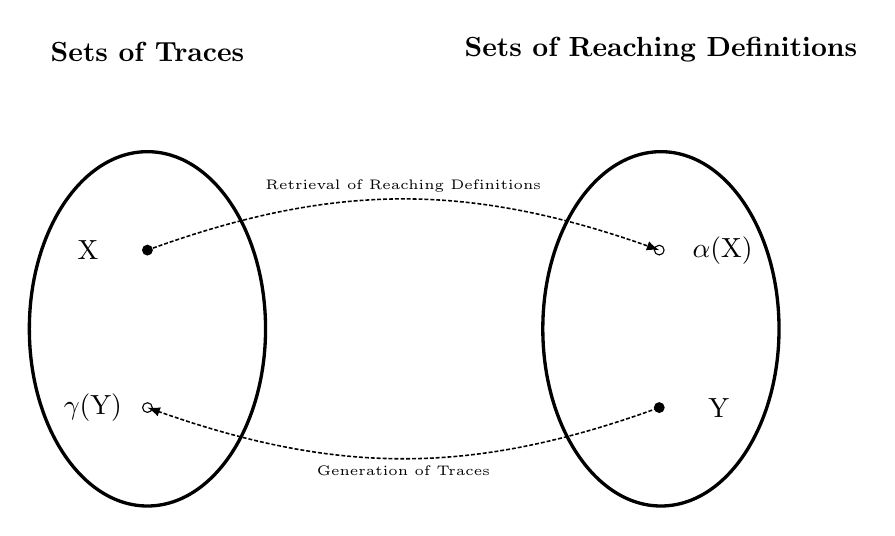
\begin{tikzpicture}
					[    
						longcircle/.style={ellipse, draw=black!100, fill=green!0, very thick, minimum width = 3cm, minimum height = 4.5cm},
						rectanglenode/.style={rectangle, draw=cyan!60, fill=cyan!20, very thick, minimum width=30mm, minimum height = 10mm},
						transparentbox/.style={rectangle,draw=blue!60, fill=blue!0, ultra thick, minimum width = 75mm, minimum height = 40mm},
					]
					
					\node[longcircle] (main) at(0,0) {} ;
					\node[longcircle] (abstract) [right=of main] at(4,0){};
		
					\node [] (texttitleconcrete) [above=of main]{{\bfseries Sets of Traces}};
					\node [] (texttitleabstract) [above=of abstract]{{\bfseries Sets of Reaching Definitions}};
					
		
					\tkzDefPoint(0,1){traces}
					\tkzDefPoint(0,-1){reach}
					
					\tkzDrawPoints[color=black,shape=circle,fill=black,size=3.5](traces)
					\tkzDrawPoints[color=black,shape=circle,fill=black!0,size=3.5](reach)
					
					\tkzDefPoint(6.5,1){traces1}
					\tkzDefPoint(6.5,-1){reach1}
					
					\tkzDrawPoints[color=black,shape=circle,fill=black,size=3.5](reach1)
					\tkzDrawPoints[color=black,shape=circle,fill=black!0,size=3.5](traces1)
					
					\tiny
					\draw[-latex,line width=0.20mm,dashed,dash pattern=on 0.5mm off 0.25mm] (traces.140) to[bend left=(20)] node[above]{Retrieval of Reaching Definitions} (traces1.39);
					\draw[latex-,line width=0.20mm,dashed,dash pattern=on 0.5mm off 0.25mm] (reach.140) to[bend left=(-20)] node[below] {Generation of Traces} (reach1.39);
					\normalsize
		
					\node [] (xtext) [left=of traces] at(0.5,1) {X};
					\node [] (ytext) [left=of reach] at(0.8,-1) {$\gamma$(Y)};
					
					\node [] (xtext1) [right=of traces1] at(5.8,1) {$\alpha$(X)};
					\node [] (ytext1) [right=of reach1] at(6,-1) {Y};
		
		
				\end{tikzpicture}
		
				\caption{Realization of Galois Connection}
				\label{fig:realgaloisconnect}
			\end{figure}
		
		\subsection*{Induced Analysis}
		\par Finally, an induced analysis is performed on the information obtained, providing a calculated analysis of the previously undecidable properties, as shown in
		Figure \ref{fig:eptc_abstraction}. This type of analysis provides a result which is produced efficiently, and relatively precisely.
	
		\begin{figure}
			\centering
			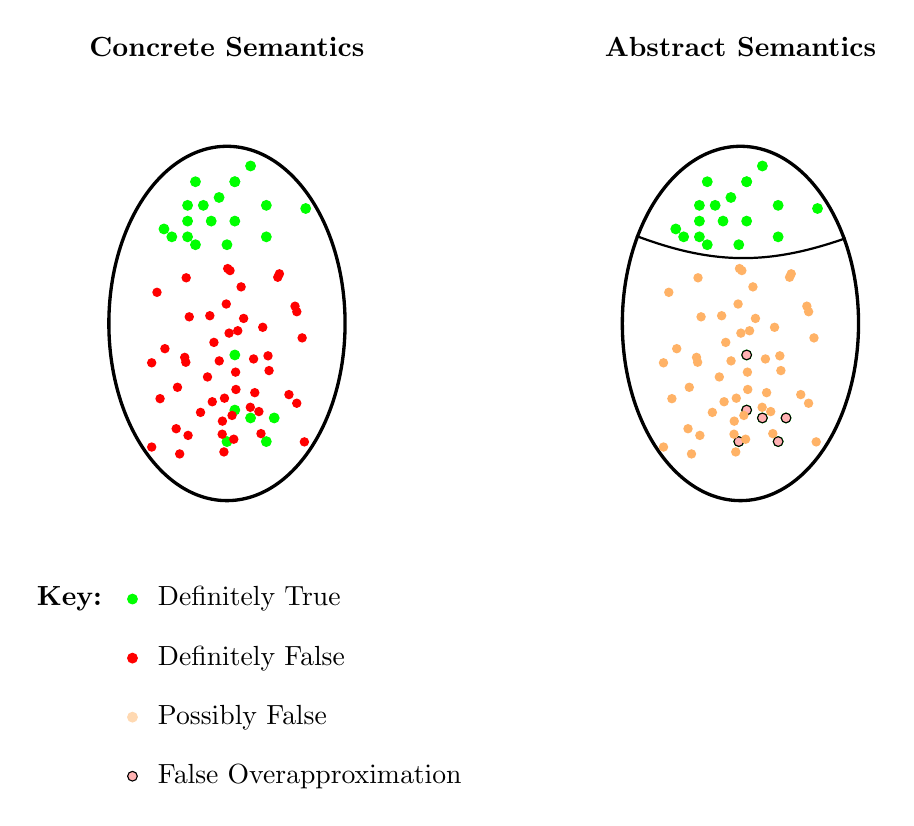
\begin{tikzpicture}
				[
					ellipsenew/.style={ellipse, draw=black!100, fill=green!0, very thick, minimum width = 3cm, minimum height = 4.5cm},
					rectanglenode/.style={rectangle, draw=cyan!60, fill=cyan!20, very thick, minimum width=30mm, minimum height = 10mm},
					transparentbox/.style={rectangle,draw=blue!60, fill=blue!0, ultra thick, minimum width = 75mm, minimum height = 40mm},
				]
	
				\node[ellipsenew] (main) at(0,0) {} ;
				\node[ellipsenew] (abstract) [right=of main] at(4,0){};
				
				%% MAIN ELLIPSE
				\pgfmathsetseed{24122015}
				\begin{scope}
					\tkzDefPoint(0,1){A}
					\tkzDefPoint(0.3,2){B}
					\tkzDefPoint(-0.2,1.3){C}
					\tkzDefPoint(-0.1,1.6){D}
					\tkzDefPoint(1,1.46){E}
					\tkzDefPoint(0.1,1.8){F}
					\tkzDefPoint(0.1,1.8){G}
					\tkzDefPoint(-.4,1.8){H}
					\tkzDefPoint(-0.3,1.5){I}
					\tkzDefPoint(0.5,1.1){J}
					\tkzDefPoint(-0.5,1.1){K}
					\tkzDefPoint(0.5,1.5){L}
					\tkzDefPoint(-0.5,1.5){M}
					\tkzDefPoint(-0.5,1.3){N}
					\tkzDefPoint(-0.7,1.1){O}
					\tkzDefPoint(-0.4,1){P}
					\tkzDefPoint(-0.8,1.2){Q}
					\tkzDefPoint(0.5,-1.5){R}
					\tkzDefPoint(0.3,-1.2){S}
					\tkzDefPoint(0.1,-1.1){T}
					\tkzDefPoint(0.6,-1.2){U}
					\tkzDefPoint(0.1,-0.4){V}
					\tkzDefPoint(0.1,1.3){W}
					\tkzDefPoint(0,-1.5){X}
					\tkzDrawPoints[color=green,shape=circle,fill=green,size=3.5](A,B,C,D,E,F,G,H,I,J,K,L,M,N,O,P,Q,R,S,T,U,V,W,X)
				\end{scope}
							
				\begin{scope}[yshift=-0.5cm]
					\pgfmathsetseed{24122015}
					%\clip(0,0) ellipse (1.5 and 4.5);
					%\clip(0,4) ellipse (1.5 and 4.5);
					\foreach \p in {1,...,50}
					{ 
						\fill[red] (1*rand,1.2*rand) circle (0.06);
					}
					
				\end{scope}
	
				%% ABSTRACT ELLIPSE
	
				\begin{scope}[xshift=6.5cm]
					\tkzDefPoint(0,1){A}
					\tkzDefPoint(0.3,2){B}
					\tkzDefPoint(-0.2,1.3){C}
					\tkzDefPoint(-0.1,1.6){D}
					\tkzDefPoint(1,1.46){E}
					\tkzDefPoint(0.1,1.8){F}
					\tkzDefPoint(0.1,1.8){G}
					\tkzDefPoint(-.4,1.8){H}
					\tkzDefPoint(-0.3,1.5){I}
					\tkzDefPoint(0.5,1.1){J}
					\tkzDefPoint(-0.5,1.1){K}
					\tkzDefPoint(0.5,1.5){L}
					\tkzDefPoint(-0.5,1.5){M}
					\tkzDefPoint(-0.5,1.3){N}
					\tkzDefPoint(-0.7,1.1){O}
					\tkzDefPoint(-0.4,1){P}
					\tkzDefPoint(-0.8,1.2){Q}
					
					\tkzDefPoint(0.5,-1.5){R}
					\tkzDefPoint(0.3,-1.2){S}
					\tkzDefPoint(0.1,-1.1){T}
					\tkzDefPoint(0.6,-1.2){U}
					\tkzDefPoint(0.1,-0.4){V}
					
					\tkzDefPoint(0.1,1.3){W}
					
					\tkzDefPoint(0,-1.5){X}
	
					\tkzDrawPoints[color=green,shape=circle,fill=green,size=3.5](A,B,C,D,E,F,G,H,I,J,K,L,M,N,O,P,Q,R,S,T,U,V,W,X)
					\tkzDrawPoints[color=black,shape=circle,fill=red!30,size=3.5](R,S,T,U,V,X)
				\end{scope}
	
				\begin{scope}[yshift=-0.5cm, xshift=6.5cm]
					\pgfmathsetseed{24122015}
					%\clip(0,0) ellipse (1.5 and 4.5);
					%\clip(0,4) ellipse (1.5 and 4.5);
					\foreach \p in {1,...,50}
					{ 
						\fill[orange!60] (1*rand,1.2*rand) circle (0.06);
					}
					
				\end{scope}
	
				
				\node [] (texttitleconcrete) [above=of main]{{\bfseries Concrete Semantics}};
				\node [] (texttitleabstract) [above=of abstract]{{\bfseries Abstract Semantics}};
	
				\draw[thick] (abstract.140) to[bend left=(-20)] (abstract.39);
				
				%% KEY
				\begin{scope}
					\node[] (key) at(-2,-3.5) {{\bfseries Key:}};
					\node[] (dtrue) [right=of key] at(-2,-3.5) {Definitely True};
					\node[] (dfalse) [right=of key] at(-2,-4.25) {Definitely False};
					\node[] (pfalse) [right=of key] at(-2,-5) {Possibly False};
					\node[] (pfalse) [right=of key] at(-2,-5.75) {False Overapproximation};
	
					\tkzDefPoint(-1.2,-3.5){TESTPOINT_TRUE}
					\tkzDefPoint(-1.2,-4.25){TESTPOINT_FALSE}
					\tkzDefPoint(-1.2,-5){TESTPOINT_POSFALSE}
					\tkzDefPoint(-1.2,-5.75){TESTPOINT_FALSENEGATIVE}
					\tkzDrawPoints[color=green,shape=circle,fill=green,size=3.5](TESTPOINT_TRUE)
					\tkzDrawPoints[color=red,shape=circle,fill=red,size=3.5](TESTPOINT_FALSE)
					\tkzDrawPoints[color=orange!30,shape=circle,fill=orange!30,size=3.5](TESTPOINT_POSFALSE)
					\tkzDrawPoints[color=black,shape=circle,fill=red!30,size=3.5](TESTPOINT_FALSENEGATIVE)
	
				\end{scope}
				
			\end{tikzpicture}
			\caption{Efficiency-Precision trade-off presented by Abstraction Interpretation}
			\label{fig:eptc_abstraction}
		\end{figure}
	
		\pagebreak
		\subsection{Type and Effect Systems}
		\label{subsec:typeeffectsys}
		\par Type and effect systems are the amalgamation of both an Effect System and an Annotated Type System \cite[pp.17--18]{nielson2004principlesofPA}.
		In an Effect System information about what happens when an execution occurs, rendering a change the current state, is produced (ex: what exception might be raised if this execution occurs).
		In an Annotated Type system the judgements that occur describe certain properties of states, such as a variables signum. Further detail into this method of analysis will not be delved into,
		as it is out of this papers scope. A simple Type and Effect listing may be seen in Listing \ref{lst:smlcodesnippet}.
		
		\begin{tikzpicture}[remember picture]
			\node(code) [anatomy] at (0,0){
				\begin{lstlisting}[caption=Type \& Effect System example on SML Code Snippet, language=ML,label=lst:smlcodesnippet]
					!*\mtPoint{mostLeft}*!let val !*\cPart{localVar1}{ref}*! = !*\cPart{localVar2}{reference (fn x=>x)}*!
					in {!*\cPart{localVar3}{ref}*! := (fn n=>n+1);                    
						!ref true    
						}
					end !*\mbPoint{mostBottom}*!
				\end{lstlisting}
			};

			\codeAnnotation{varText1} (3,5) {TYPE: int$\rightarrow$int reference}
			\codeAnnotation{effecttext} (9,5) {EFFECT: creates an int$\rightarrow$int reference}
			\codeAnnotation{text3} (7,2.5) {int$\rightarrow$int reference}

			\draw[->,annotation](varText1) -- (localVar1);
			\draw[->,annotation](effecttext) -- (localVar2);
			\draw[->,annotation](text3) -- (localVar3);

		\end{tikzpicture}
    \chapter{Methodology}
    \par This chapter describes how the \nameref{sec:propsol} was implemented, and why certain decisions were taken regarding design implementation. This chapter also explores the problems encountered whilst formulating such a design.
    %%TODO: finish section
    \section{Initial Challenges}
    \par The effects that CPython Bytecodes have on the CPython stack are not explicitly defined; posing as an initial challenge. CPython also implements certain bytecode optimizations, initially hindering the ability to fully understand
    the operations taking place in relation to the source code. Official Python documentation is very vague, intertwining terminologies making it difficult to understand the inner workings of the \acs{PVM}.
    \section{Abstract Design}
    \par PATH is a three-phase bytecode inspection tool (Sections \ref{subsec:phaseoverview} \& \ref{sec:concimp} respectively). The high-level implementation is as follows; 
    PATH iteratively inspects each bytecode instruction produced by the Python Compiler, generating facts as instructions are iterated through. 
        \subsection{Phase Overview}
        \label{subsec:phaseoverview}
        \begin{itemize}
            \item[1.] The preliminary phase is the setup phase. This phase tackles the initialization of all the global variables required for bytecode inspection along with the statement relations.
            \item[2.] The second phase is the iteration phase; \acs{AIL}. This phase is where the main logic of the framework is found. The manipulation of local and global variables, pertaining to the IR and fact generation also occurs in this phase.
            \item[3.] The third and final phase generates a block summary, by retrieving information from the generated facts in phase 2.   
        \end{itemize}
        
        \begin{figure}
            \centering

            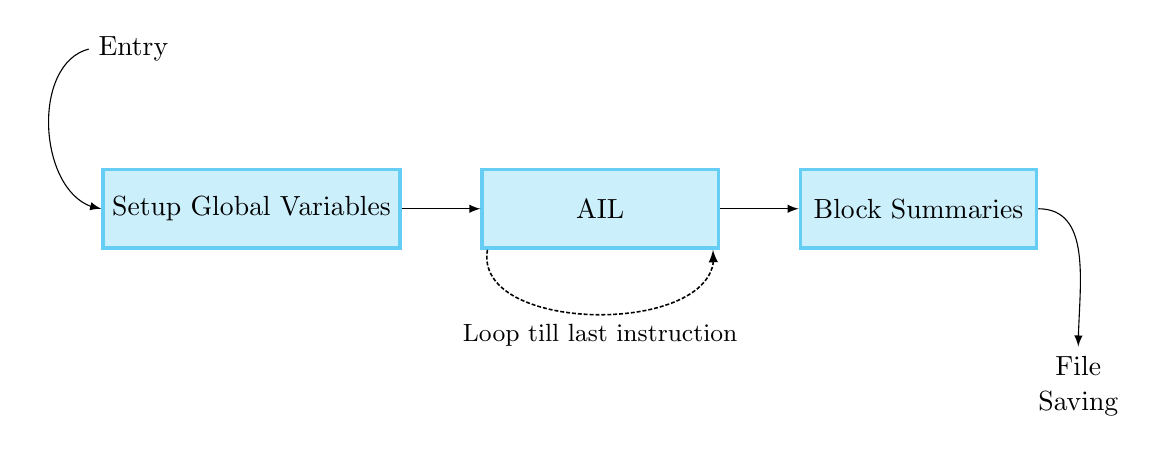
\begin{tikzpicture}
					[
						roundnode/.style={circle, draw=green!60, fill=green!5, very thick, minimum size=20mm},
						rectanglenode/.style={rectangle, draw=cyan!60, fill=cyan!20, very thick, minimum width=30mm, minimum height = 10mm},
						transparentbox/.style={rectangle,draw=blue!60, fill=blue!0, ultra thick, minimum width = 75mm, minimum height = 40mm},
					]
                    
                    
                    \node[rectanglenode] (main) at (0,0) {Setup Global Variables};
                    \node[rectanglenode] (bil) [right=of main] {\acs{AIL}};
                    \node[rectanglenode] (bs) [right=of bil] {Block Summaries};
                    
                    \node[] (entrytext) [above=of main] at(-1.5,0.75) {Entry};
                    \node[] (filesavetext) [below=of bs] at(10.5,-0.75) {File};
                    \node[] (savetext) [below=of bs] at(10.5,-1.2) {Saving};
                    
                    \draw[-latex] (main.east) -- (bil.west);
                    \small
                    \draw[-latex,line width=0.20mm,dashed,dash pattern=on 0.5mm off 0.25mm] (bil.200) to[bend left=(-100)] node[below]{Loop till last instruction} (bil.340);
                    \normalsize
                    \draw[-latex] (bil.east) -- (bs.west);

                    \draw[-latex] (entrytext.west) to[bend left=-80] (main.west);
                    \draw[-latex] (bs.east) to[out=0, in=90] (filesavetext.north);
                    

            \end{tikzpicture}

            \caption{Phases of \acs{PATH}}
            \label{fig:pathphases}
        \end{figure}

    \section{Concrete implementation}
    \label{sec:concimp}
        \subsection{Setup}
            \par The setup stage is the entry point to the framework. This stage is simple; setting up of the basic variables, which provide a basis for the upcoming logic of \acs{PATH}.
            \subsubsection*{Relation Initialization}
            \par The first stage deals with the initialization of the \textit{Statement Relations}; imperative for fact generation.
            Most of the relations are initially realized as sets. Lists are only used for the relations which are required to be stored in an ordered fashion. This requirement is motivated 
            by the relations dependency, so as to achieve proper internal fact generation. These relations are \lstinline{simple_statement_ir}, \lstinline{statement_uses_local}, and \lstinline{statement_uses_global}.
            By design, as one reaches the termination of \acs{PATH}, these relations are consolidated into a Python dictionary; returned as \lstinline{fact_dict}. An in-depth review of all relations is found in Section \ref{sec:factgen}

            \subsubsection*{Global Variable Initialization}
            \par Following the initialization of the relations, the \textit{Global Variables} are conceived. These variables are used throughout \acs{PATH}, namely for proper block and instruction variable handling, thus
            are divided into two main distinct groups; Global Instruction Variables, and Global Block Variables. Any other variables are classified as Miscellaneous Variables. All Global Variables are initialized as empty variables, unless said otherwise.

        \subsection{\acs{AIL}}
        \label{subsec:AILimp}
        \par An abundant amount of the framework's logic is packed into the \acs{AIL}. This loop iterates through every bytecode instruction, recording attributes of the instruction, and how 
        each instruction interacts with the previous instruction, and will interact with the next instruction. The iterative nature (known as \acs{III}) of the \acs{AIL} was inspired by the Python VM Innards workings (See Figure \ref{fig:vm_innards}). Inspecting the bytecodes in such a fashion (i.e. generating all the facts iteratively) is arguably faster than having 
        a phase per fact needed to be generated. In addition to fact generation, we also incorporated \acs{CFA} and \acs{IR} generation in the \acs{III} fashion; taking a different approach to how current inspection tools operate (such as Pylint), whereby first the \acs{IR} is generated, following an analysis conducted on the \acs{IR} itself. This is a multiphase process, in comparison to the single phase 
        design created by \acs{AIL}.
            \subsubsection*{Bytecode Validity}
            Firstly, bytecode instruction validity is ensured via the specified opcode dictionary (supported Bytecode Instructions can be found in \nameref{table:opcode_table}).
            \subsubsection*{Local Variable Initialization}
            \par Following verification, local instruction variables are set. These variables are the first to be set as they are the basis for fact generation and block generation. These variables are also the foundation for the \acs{IR} generated, namely for setting the instruction line number 
            and the instruction identifier. The former is dynamically set, dependent on the amount of opcodes that need to be processed, whilst the latter is generated by a specially designed \acs{MD5} algorithm, creating parameter dependent unique hashes for every instruction.
            \subsubsection*{Block Handling}
            \par Block handling is the subsequent step, modifying the local block variables. In \acs{PATH} the notion of a [elementary] block is a primitive from which a program is constructed by. Entry and exit points of blocks depend on the current program flow (as seen in Section \ref{subsec:dfa}); they form part of the 
            basis of both \acs{DFA} and \acs{CFA}. New blocks are uniquely identified (similarly to the instruction identifier) and instructions are bound to their respective block (as is seen in Section \ref{sec:factgen}). By design, each block
            has its own stack and unique properties (see Section \ref{sec:cfimp}) that are used as a basis for both fact generation and accurate block analysis.
            \par An interesting design feature of \acs{AIL} is the incorporation of both Block Handling and Control Flow Analysis in one sub-phase. Moreover, this sub-phase is only executed if an instruction forms part of a new block; avoiding redundant execution stages.  
            \subsubsection*{Opcode Handling}
            \par This stage handles general opcode tasks (i.e: general relation generation) and opcode specific tasks (i.e: recursive \lstinline|MAKE_FUNCTION| dictionary nesting). There exist opcodes, such as \lstinline|MAKE_FUNCTION| which require additional parameters to be considered for accurate fact generation. The incorporation of the opcode specific \acs{IR} generation in this stage, expedites the process of fact and IR generation, compared to 
            having the \acs{IR} generated in a separate stage.
            \subsubsection*{\acs{IR} Handling}
            \par The penultimate process is the \acs{IR} Generation stage. This stage handles the \acs{IR} generation according to the current opcode. \acs{IR} generation is further delved into in Section \ref{sec:irgen}.
            \subsubsection*{Updating Global Variables}
            \par The final stage in the \acs{AIL} simply updates the global variables that are to be used in the next iteration.

        \subsection{Block Summary}
        \par The termination of \acs{PATH} is brought about by the block summaries, conducted on the facts generated in the \acs{AIL}. A block summary is generated for every block, showing where blocks start and end; useful for external debugging purposes and instruction grouping. The generation of a block summary is a form of block analysis. 

            
    \section{Fact Generation} \label{sec:factgen}
    \par In \acs{PATH} a fact is information which is generated from the program that is being inspected. These facts are useful for end users as they provide deeper insight in the operations that occur in the program, reducing the overall engineering complexity of program analysis. \acs{PATH} produces three types of facts: Statement facts, Block facts, and Program facts.
    Facts are generated in \acs{III} fashion (per bytecode instruction) and outputted to the user as \textit{.fact} files. A table of all the facts and their descriptions is found in the \nameref{table:facts_table}. 

    \section{Control Flow} \label{sec:cfimp}
    \par Control Flow in \acs{PATH} is implemented within the block handling stage in \acs{III} fashion, as mentioned in Section \ref{subsec:AILimp}. The block handling stage is broken down in three main parts; block variable generation, control flow handling and block \acs{I/O}.
        \subsubsection*{Block Variable Generation}
        \par Block variables are only generated if the start of a new block is detected. New blocks are based on jumps and labels, whereby a new block starts after a jump instruction or at a label. The latter is a jump target (i.e: which bytecode a jump instruction would jump to) and the former is self-explanatory. 
        The detection of a new block triggers the block variables to be generated along with certain facts pertaining to block information.    
        

        \begin{lstlisting}[float=h,language=Python,caption= Conditional statement script,label=lst:condscriptLIst]
            if x>3:
                #do something#
            else:
                #do something else#
        \end{lstlisting}

        \begin{tikzpicture}[remember picture]
            \node(code) [anatomy] at(0,0) {
            \begin{lstlisting}[language=bash,caption= Bytecode Dissasmbly of Listing \ref{lst:condscriptLIst},numbers=none]
            1           0 LOAD_GLOBAL              0 (x)
                        2 LOAD_CONST               1 (3)
                        4 COMPARE_OP               4 (>)
                        6 !*\cPart{jumpinst1}{POP\_JUMP\_IF\_FALSE}*!       10

            2           8 !*\cPart{jumpinst2}{JUMP\_FORWARD}*!             0 (to 10)

            4     !*\cPart{varlab}{>>}*!   10 LOAD_CONST               0 (None)
            12          RETURN_VALUE
            \end{lstlisting}
            };

            \codeAnnotation{varText1} (2,2.8) {Label}
            \codeAnnotation{varText2} (12,2.8) {Jump Instruction}
            \codeAnnotation{varText3} (3,4) {Jump Instruction}

            \draw[->,annotation](varText1) -- (varlab);
            \draw[->,annotation](varText2) -- (jumpinst2);
            \draw[->,annotation](varText3) -- (jumpinst1);
        \end{tikzpicture}

        \subsubsection*{Control Flow Generation}
        \par Following the initialization, links between the edges of basic blocks are generated; as shown in Figure \ref{fig:cfhandling}. It is ensured that upon encountering a jump, no redundant relations are created between blocks; taking care to only create relations between linked block edges (i.e: a block's \textit{if} block cannot enter the same \textit{else} block). These type 
        of relations are avoided by creating a unique identifier (\lstinline|block_link_id|); uniquely identifying a link between two blocks.

        \begin{figure}[H]
            \centering
            \tiny
            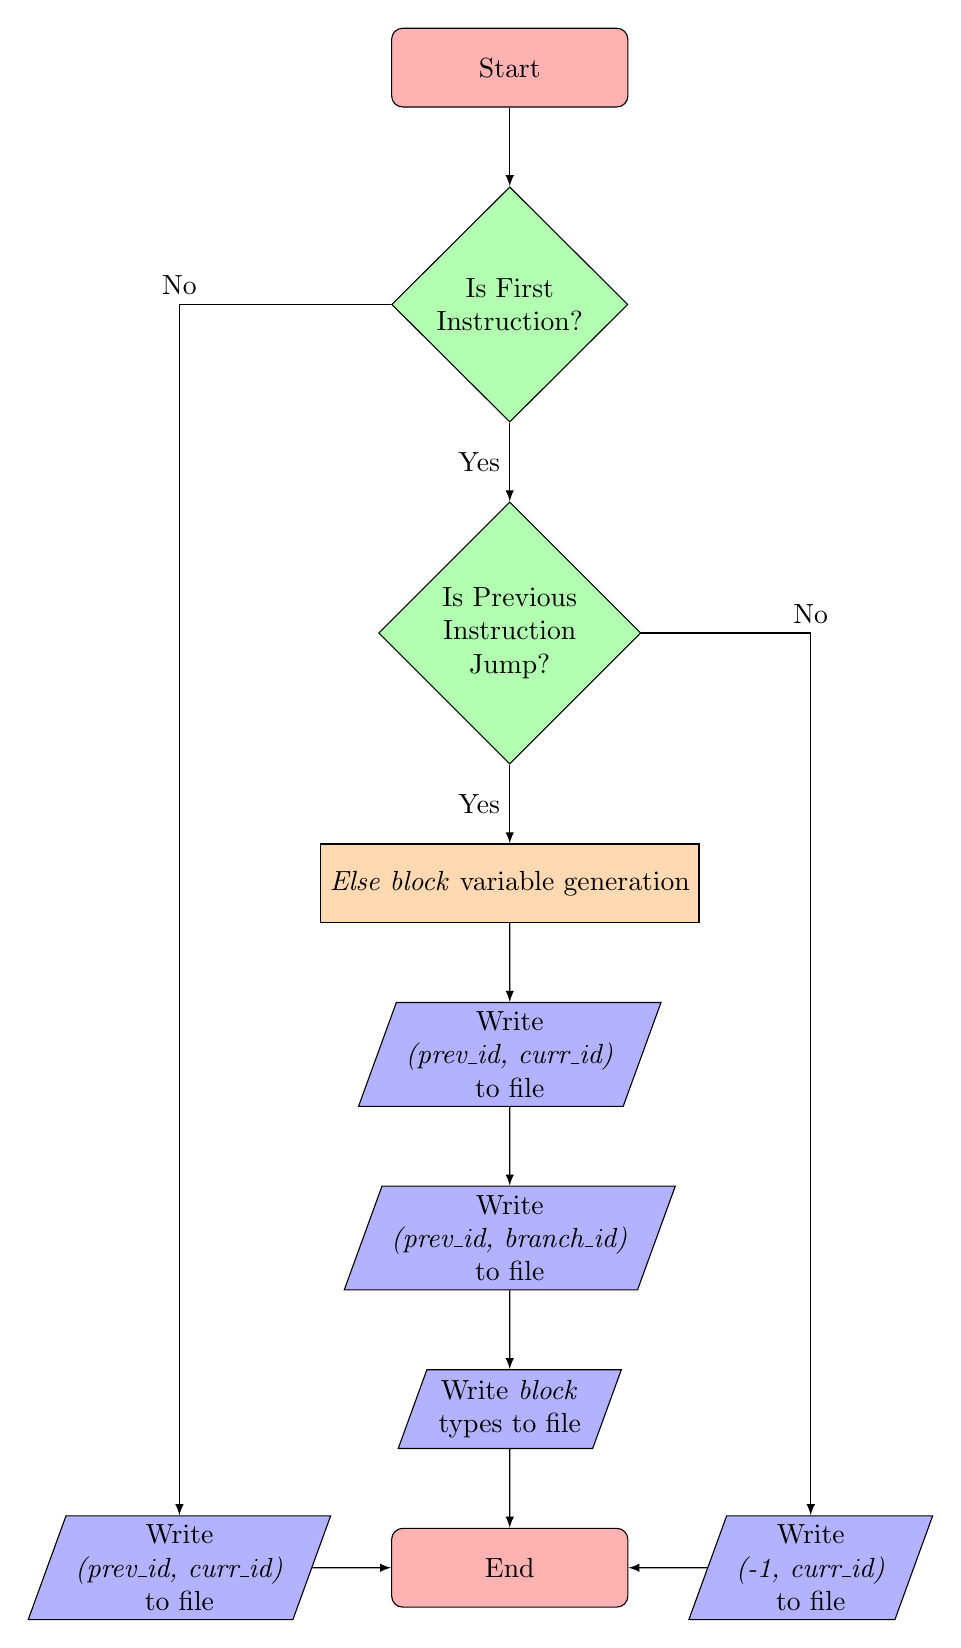
\begin{tikzpicture}
                [
                    roundnode/.style={circle, draw=green!60, fill=green!5, very thick, minimum size=20mm},
                    rectanglenode/.style={rectangle, draw=cyan!60, fill=cyan!20, very thick, minimum width=30mm, minimum height = 10mm},
                    transparentbox/.style={rectangle,draw=blue!60, fill=blue!0, ultra thick, minimum width = 75mm, minimum height = 40mm},    
                    startstop/.style={rectangle, rounded corners, minimum width=3cm, minimum height=1cm,text centered, draw=black, fill=red!30},
                    process/.style= {rectangle, minimum width=2cm, minimum height=1cm, text centered, draw=black, fill=orange!30},
                    decision/.style = {diamond, minimum width=3cm, minimum height=.5cm, text centered, draw=black, fill=green!30,align=center},
                    io/.style = {trapezium, trapezium left angle=70, trapezium right angle=110, minimum width=2cm, minimum height=1cm, text centered, draw=black, fill=blue!30, align=center}
                ]
                
                \node [startstop] (entry) {Start};
                \node [decision] (1stdes) [below=of entry] {Is First \\ Instruction?};
                \node [decision] (2nddes) [below=of 1stdes] { Is Previous \\ Instruction \\Jump?};
                \node [process] (1stproc) [below= of 2nddes] {\textit{Else block} variable generation};
                \node [io] (2ndio) [below= of 1stproc] {Write \\ \textit{(prev\_id, curr\_id)} \\ to file};
                \node [io] (3rdio) [below= of 2ndio] {Write \\  \textit{(prev\_id, branch\_id)} \\ to file};
                \node [io] (4thio) [below= of 3rdio] {Write \textit{block} \\ types to file};
                \node [startstop]  [below=of 4thio] (end) {End};
                
                \node [io] (5thio) [left= of end] {Write \\  \textit{(prev\_id, curr\_id)} \\ to file};
                \node [io] (6thio) [right= of end] {Write \\  \textit{(-1, curr\_id)} \\ to file};
                

                \draw [-latex] (entry) -- (1stdes);
                \draw [-latex] (1stproc) -- (2ndio);
                \draw [-latex] (2ndio) -- (3rdio);
                \draw [-latex] (3rdio) -- (4thio);
                \draw [-latex] (4thio) -- (end);
                \draw [-latex] (5thio) -- (end);
                \draw [-latex] (6thio) -- (end);

                \draw [-latex] (1stdes) -- node[anchor=east] {Yes} (2nddes);
                \draw [-latex] (2nddes) -- node[anchor=east] {Yes} (1stproc);

                \draw [-latex] (1stdes) -| node[anchor=south] {No} (5thio);
                \draw [-latex] (2nddes) -| node[anchor=south] {No} (6thio);
                
            \end{tikzpicture}
            \caption{Control Flow Handling}
            \label{fig:cfhandling}
        \end{figure}

        \section{\acs{IR} Generation}
        \label{sec:irgen}
        \par The \acs{IR} that \acs{PATH} creates is intended to reduce the engineering complexity for further program analysis. The complex task of recording variables that are consumed and created in a more concise form
        was needed, so as to resolve the tedious task of manually keeping note of all stack operations. \acs{PATH} currently offers this functionality for three primary operation subtypes:
        \begin{enumerate}
            \item Binary Operation Binding
            \item Function Calling Binding
            \item Method Loading Binding
            \item Return Value Binding
        \end{enumerate}
        Providing a standardized representation for the cases above greatly simplifies the final representation of a program. \acs{IR} generation takes a \acs{III} approach; following a sequential iterative generational pattern.
        \begin{description}
            \item[Binary Operation Binding] takes the arguments from a binary operation (see \nameref{table:opcode_table}), binding them to the variable specified, summarizing a binary operation as shown in Listing \ref{lst:binopIR}.
            
            \begin{lstlisting}[language=bash,caption=Binary Operation Binding Syntax w/variable,numbers=none,label=lst:binopIR]
<inst_id> <var_id> = <inst_name> <arg1> <operation> <arg2>
            \end{lstlisting}

            Binary operations which do not have a variable bound to them produce the \acs{IR} shown in Listing \ref{lst:binopIRnovar}

            \begin{lstlisting}[language=bash,caption=Binary Operation Binding Syntax w/no variable,numbers=none,label=lst:binopIRnovar]
<inst_id> <inst_name> <arg1> <operation> <arg2>
            \end{lstlisting}

            \item[Function Calling Binding] takes the function and arguments passed to the said function, binding them to the function identifier, indicated by a succeeding \lstinline|STORE_FAST| instruction. This is shown below.
            \begin{lstlisting}[language=bash, caption=Function Calling Binding,numbers=none]
<inst_id> <func_id> CALL_FUNCTION <function_name><arg1> ... <argN>
            \end{lstlisting}
        
            \item[Method Loading Binding] takes any \lstinline|LOAD_METHOD| calls, merging them with the arguments of its respective \lstinline|CALL_METHOD|. The latter instruction indicates the number of positional arguments that are passed to the method loaded by the former instruction. 
            \begin{lstlisting}[language=bash, caption=Method Loading Binding,numbers=none]
<inst_id><func_id>LOAD_METHOD<function_name><arg1>...<argN>
            \end{lstlisting}
            \item[Return Value Binding] simply represents the return value bound with its instruction identifier.
            \begin{lstlisting}[language=bash, caption=Function Calling Binding,numbers=none]
                <inst_id> RETURN_VALUE <arg1>
            \end{lstlisting}
        \end{description}



    \section{Technical Implementation}
            
           \par The technical implementation is documented within the source code, as inline comments.
    \chapter{Evaluation}
    In this chapter \acs{PATH} is tested and evaluated. For testing, programs with varying complexity are used; simple programs ranging to more complex programs. 
    There are three primary \nameref{sec:researchque}, which will be tested in Sections \ref{sec:ffa}, \ref{sec:ins} and \ref{sec:scalex}; validating \acs{PATH}.

    \section{Research Questions}
    \label{sec:researchque}
        The research questions below systematically investigate the need and use of \acs{PATH}. These questions are delved into more depth in Sections \ref{sec:ffa}, \ref{sec:ins}, and \ref{sec:scalex}.
        
        \begin{description}
            \item[RQ 1: How is further analyses facilitated?] \acs{PATH} creates \textit{.facts} files. Such files contain metrics pertaining to the function analysed that are of interest to end users.
            These files' contents are tabulated in \nameref{table:facts_table}.
            \item[RQ 2: What findings are concluded from this project?] Throughout this project, several undocumented findings have been concluded from results generated by \acs{PATH} processing the functions in \textit{project/tests}.
                The primary undocumented findings are listed below:
                \begin{itemize}
                    \item Elementary Blocks in CPython retain their content on the frame stacks, propagating through the blocks.
                    \item \lstinline|LOAD_GLOBAL| is reserved for storing function names.
                    \item Bytecode operations on the frame stack. 
                    \item CPython blocks are not elementary blocks.
                \end{itemize}
                These findings amongst others are further discussed in Section \ref{sec:ins}.
            
            \item[RQ 3: Is \acs{PATH} scalable?] For \acs{PATH} to be of any practical use, it must be able to scale appropriately, and traverse through different function calls.  
            This is possible as it follows a recursive methodology when dealing with \lstinline|MAKE_FUNCTION| calls, and also scales linearly in relation to the number of bytecodes in a function.

        \end{description}

    \section{Facilitating further analyses}
    \label{sec:ffa}
    \par Program analysis is a computationally intensive and time-consuming process. This process is facilitated by the use of automated tools, such as \acs{PATH}. The \textit{facts} generated 
    by \acs{PATH} are thought out in such a way so as to analyse functions and to enable any further analyses, such as carrying out a Data Flow Analysis with the 
    information generated by \acs{PATH}. For a Data Flow Analysis one requires a \acs{CFG} (generated as mentioned in Section \ref{sec:cfimp}), and data-flow equations for every node of the \acs{CFG}.
    A popular approach to Data Flow Analysis is the Reaching Definitions Method (See section \ref{subsec:dfa}). This would be facilitated with \acs{PATH} via the \acs{CFG} generated and the following \textit{.facts} files:
    \textit{StatementUsesLocal.facts} and \textit{PushValue.facts} (refer to \nameref{table:facts_table}); demonstrating that it does indeed reduce the engineering complexity of further analysis. 
    \par This tool enables teams to focus on the analysis itself, negating the preliminary step for the creation of different intermediary representations which analysis is conducted on. The lack of professionals in this area makes complex analysis tools expensive and rare to come across.
        \subsection{Relating \acs{PATH} with current frameworks}
            \par In reality, program analysis cannot be simply bisected into two categories; it is more accurately depicted by the scope shown in Figure \ref{fig:spectrumPA}

            \begin{figure}
                \centering
                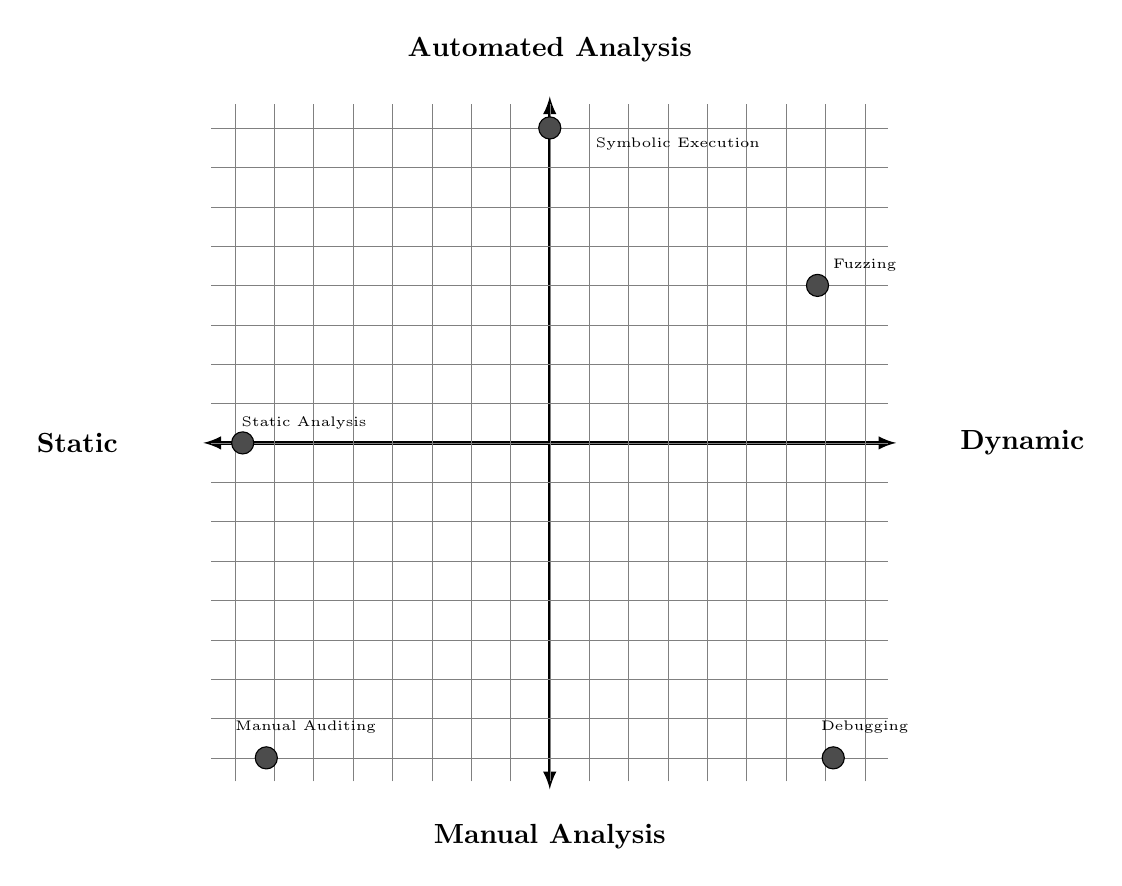
\begin{tikzpicture}
                    
                    \node[align=center] (staticstring) at(-6,0){ \bfseries{Static}};
                    \node[align=center] (Dynamicstring) at(6,0){ \bfseries{Dynamic}};
                    \node[align=center] (autostring) at(0,5){ \bfseries{Automated Analysis}};
                    \node[align=center] (manual) at(0,-5){ \bfseries{Manual Analysis}};

                    %%axis
                    \draw[very thick,latex-latex] (-4.4, 0) -- (4.4, 0);
                    \draw[very thick,latex-latex] (0, -4.4) -- (0, 4.4);
                    
                    %%background
                    \draw[ultra thin, gray, step=.5cm] (-4.3,-4.3) grid (4.3,4.3);

                    \tkzDefPoint(-3.9,0){static}
                    \tkzDefPoint(0,4){symEx}
                    \tkzDefPoint(-3.6,-4){manual}
                    \tkzDefPoint(3.4,2){dynamic}
                    \tkzDefPoint(3.6,-4){debug}
                    \tkzDrawPoints[color=black,shape=circle,fill=black!70,size=8](static,symEx,manual,dynamic,debug);
                    
                    \tiny
                    \node[] (text1)[right=of static] at (-5,0.25) {Static Analysis};
                    \node[] (text2)[right=of static] at (-0.5,3.8) {Symbolic Execution};
                    \node[] (text3)[below=of static] at (-3.1,-2.45) {Manual Auditing};
                    \node[] (text4)[below=of debug] at (4,-2.45) {Debugging};
                    \node[] (text4)[above=of dynamic] at (4,1.1) {Fuzzing};

                    \normalsize

                \end{tikzpicture}
                \caption{Scope of Program Analysis}
                \label{fig:spectrumPA}
            \end{figure}
            \subsubsection*{Similar Frameworks}
            \par \acs{PATH} is a pure basic program analysis framework, in which its stereobate lies with the generation of an \acs{IR}. This framework takes inspiration from several other
            Static frameworks which operate similarly:
            \begin{description}
                \item[doop]A Java pointer and Taint Analysis framework that conducts analysis by the Soufflé Datalog Engine \cite[]{bravenboer2009strictly}.
                \item[soot]A Java optimization framework, providing analyses ranging from \acs{CFG} construction to Taint analysis \cite[]{vallee2010soot}.
                \item[Gigahorse]An Ethereum analysis framework, specializing in the decompilation of smart contracts \cite[]{grech2019gigahorse}.
                \item[Vandal]A fast and robust security analysis framework for Ethereum smart contracts \cite[]{brent2018vandal}.
            \end{description}
            \par The frameworks mentioned above are {\bfseries pure} program analysis frameworks (Static Analysis), whereby the analysis is conducted on an \acs{IR}.
            
            \subsubsection*{Alternative Frameworks}
            \par As seen in Figure \ref{fig:spectrumPA}, there are different methods by which program analysis can be conducted. A popular alternative to the Static Analysis Methodology is the Symbolic Execution method.
            Symbolic Execution is a technique for automatic software validation and verification; differing from Static analysis in the way that it does not form an opinion about the accuracy of the approximation generated. It is simply used to show an expected symbolic result about a computation.
            \begin{description}
                \item[Mythril] A security analysis tool for Ethereum smart contracts, following a symbolic execution methodology \cite[]{di2019survey}.
                \item[Manticore] A symbolic execution tool to analyse binaries and Etherum smart contracts \cite[]{mossberg2019manticore}. 
                \item[angr] A platform-agnostic binary analysis framework making use of a symbolic execution engine \cite[]{wang2017angr}.
                \item[Pex] A .NET white box test generation framework using a dynamic symbolic execution engine \cite[]{tillmann2008pex}.
            \end{description}


    \section{Insights}
    \label{sec:ins}
    \par This section collects the undocumented insights that have been noted from the results generated by \acs{PATH} alongside the extensive study into CPython itself.  
        \subsection{Elementary Block Behaviour}
        
        \par In CPython, an elementary block differs from a block. This is not clear in the documentation provided as one might assume that an elementary block in \acs{PA} terms is interchangeable with a CPython block. CPython considers a section of code to be a block if it is encapsulated within the following code-blocks:
        \begin{itemize}
            \item \lstinline|try| block.
            \item \lstinline|with| block.
            \item \lstinline|except| block.
            \item \lstinline|else| block.
            \item \lstinline|finally| block.
        \end{itemize}

        \par The start of a CPython block is indicated by a \lstinline|SETUP_FINALLY| instruction. The end of a CPython block, is indicated with the \lstinline|POP_BLOCK| instruction whereby all elements of the block are popped along with the block itself, shown in Listing \ref{lst:setupfinallyscript} and \ref{lst:setupfinallydis}.

        \begin{lstlisting}[float,language=Python,caption= \lstinline|try...except| script,label=lst:setupfinallyscript]
def test():
    try:
        print("Hello")
    except Exception:
        print("This is an exception")
        \end{lstlisting}

        \begin{lstlisting}[float,language=bash,caption= Excerpt Bytecode Dissasmbly of Listing \ref{lst:setupfinallyscript},label=lst:setupfinallydis,numbers=none]
            6           0 SETUP_FINALLY            7 (to 16)

            7           2 LOAD_GLOBAL              0 (print)
                        ...
                        8 POP_TOP
                       10 POP_BLOCK
                       12 LOAD_CONST               0 (None)
                       14 RETURN_VALUE
            8     >>   16 DUP_TOP
                        ...
            9          28 LOAD_GLOBAL              0 (print)
                        ...
                       40 RETURN_VALUE
            8     >>   42 RERAISE                  0
        \end{lstlisting}

        \subsection{\lstinline|LOAD_GLOBAL| versus \lstinline|LOAD_NAME|}
        \par From the results generated, it was noted that the \lstinline|LOAD_GLOBAL| instruction was used solely to look-up function names, as they cannot be local variables. Typically, the compiler compiles source code with \lstinline|LOAD_NAME| unless the variable stored is implicitly a global variable (such as a function name), or defined explicitly, as shown in Listing \ref{lst:loadglobscript}
        
        \begin{lstlisting}[float,language=Python,caption= \lstinline|LOAD_GLOBAL| script,label=lst:loadglobscript]
def foo():
    global a
    a=3
        \end{lstlisting}

        \begin{lstlisting}[float,language=bash,caption= Bytecode Dissasmbly of Listing \ref{lst:loadglobscript},numbers=none]
            3           0 LOAD_CONST               1 (3)
                        2 STORE_GLOBAL             0 (a)
                        4 LOAD_CONST               0 (None)
                        6 RETURN_VALUE
        \end{lstlisting}
    
        \subsection{Bytecode Operations}
        \par One of the most important findings that has come from the creation of \acs{PATH} is the clear, concise \nameref{table:opcode_table}. Official documentation provided by Python does not explicitly tabulate the operations on the stack performed by each instruction. CPython source code was inspected (namely \textit{ceval.c}), taking note of \lstinline|PUSH()/STACK_GROW()| and \lstinline|POP()/SHRINK()| which both grow the value stack and shrink the value stack, respectively.
        \par The creation of the \nameref{table:opcode_table} has allowed for an accurate dictionary driven implementation of the opcodes and their respective effect on the value stack in \acs{PATH}.
        
    \section{Scalability \& Experimental Results}
    \label{sec:scalex}
    
    \par Individual opcode features of \acs{PATH} were verified with basic functions found in \textit{project/tests/opcode}, logical functionality of \acs{PATH} (such as \acs{CFG} generation) was verified with 
    functions found in \textit{project/tests/logic}, and finally, general purpose testing was conducted via open source programs\footnote{obtained from \url{https://github.com/OmkarPathak/Python-Programs/tree/master/Programs}}.

    \tiny
    \begin{longtable}{|p{5cm}|p{3.5cm}|p{1cm}|p{3cm}|}
        \caption{\acs{PATH} Performance Results}
        \label{table:resultsPATH}
        \endfirsthead
        \endhead
        \hline
        \multicolumn{4}{|c|}{{\bfseries Performance Results}} \\
        \hline
        File Name::main() & Execution Time(ms) & Lines &Bytecode Length\\
        \hhline{|====|}
        P01\_hello.py & 0.34 & 1  & 10\\
        \hline
        P02\_VariableScope.py & 0.74 & 3 & 26\\
        \hline
        P03\_ListsOperations.py & 5.75 & 20 & 238\\
        \hline
        P04\_Factorial.py & 1.3 & 6 & 50\\
        \hline
        P05\_Pattern.py & 4.1 & 11 & 156\\
        \hline
        P06\_CharCount.py & 1.62 & 9 & 64\\
        \hline        
        P07\_PrimeNumber.py & 2.62 & 13 & 104\\
        \hline
        P08\_Fibonacci.py & 0.98 & 4 & 34\\ 
        \hline
        P09\_Factorial & 0.97 & 4 & 34\\
        \hline
        P10\_LCM.py & 1.69 & 8 & 58\\
        \hline
        P11\_BinaryToDecimal.py& 2.20 & 8 & 90\\
        \hline
        P12\_DecimalToBinary.py& 1.04 & 3 & 38\\
        \hline
        P13\_Palindrome.py& 1.17 & 5 & 44\\
        \hline
        P14\_CheckGreater.py& 1.31 & 6 & 50\\
        \hline
        P15\_Arguments.py& FAILED & 6 & 82\\ 
        \hline
        P16\_CountVowels.py& 1.18 & 6 & 40\\
        \hline
        P17\_EvenOdd.py& 1.65 & 8 &62\\
        \hline
        P18\_Logging.py& 1.57 & 9 & 62\\
        \hline
        P19\_SimpleStopWatch.py& 2.41 & 11 & 96\\
        \hline
        P20\_OsModule.py& 2.30 & 6 & 92\\
        \hline
        P21\_GuessTheNumber.py& 2.21 & 11 & 90\\
        \hline
        P22\_SequentialSearch.py& 1.68 & 8 & 66\\
        \hline
        P23\_BinarySearch.py& 2.83 & 14 & 104\\
        \hline
        P24\_SelectionSort.py& 2.73 & 7 & 106\\
        \hline
        P25\_BubbleSort.py& 2.71 & 4 & 100\\
        \hline
        P26\_InsertionSort.py& 2.76 & 8 & 114\\
        \hline
        P27\_MergeSort.py& 1.96 & 7 & 80\\
        \hline
        P28\_QuickSort.py& 1.42 & 6 & 54\\
        \hline
        P29\_ArgumentParser.py& 1.49 & 7 & 60\\
        \hline
        P30\_Array.py& 3.56 & 10 & 148\\
        \hline
        P31\_SinglyLinkedList.py& 3.46 & 13 & 142\\
        \hline
        P32\_Multithreading\_Client.py& 3.58 & 14 & 154\\
        \hline
        P33\_DoublyLinkedList.py& 1.97 & 7 & 80\\
        \hline
        P34\_Stack.py& 2.74 & 9 & 112\\
        \hline
        P35\_NarySearch.py& 11.25 & 40 & 422\\
        \hline
        P36\_SimpleReaderWriter.py& 2.34 & 8 & 96\\
        \hline
        P37\_HangmanGame.py&9.23 & 47& 372\\
        \hline
        P38\_HashingFile.py& 2.99 & 9 & 126\\
        \hline
        P39\_Queue.py&1.58& 7 & 64\\
        \hline
        P40\_ChiperText.py& 1.99 & 7 & 80\\
        \hline
        P41\_PortScanner.py& 1.02 & 3& 38\\
        \hline
        P42\_MultiprocessingPipes.py&2.31& 7& 96\\
        \hline
        P43\_BinarySearchTree.py&4.14 & 15&158\\
        \hline
        P44\_Closures.py& 0.89 & 5 & 10\\
        \hline
        P45\_MoreOnClosures.py&1.85 & 8 & 74\\
        \hline
        P46\_Decorators.py&1.07& 4 & 36\\
        \hline
        P47\_MoreOnDecorators.py&1.21&4&38\\
        \hline
        P48\_CountingSort.py&3.35&13&140\\
        \hline
        P49\_RockPaperScissors.py&11.39&35&434\\
        \hline
        P50\_ListComprehensions.py&10.32&36&378\\
        \hline
        P51\_PythonJSON.py&FAILED&6&62\\
        \hline
        P52\_BucketSort.py&7.54& 21&286\\
        \hline
        P53\_ShellSort.py&4.06& 11&150\\
        \hline
        P54\_PythonCSV.py&FAILED& 4 & 38\\
        \hline
        P55\_Isogram.py&1.61& 7&56\\
        \hline
        P56\_Panagram.py&2.21& 14&86\\
        \hline
        P57\_Anagram.py&1.68& 6 &66\\
        \hline
        P58\_PerfectNumber.py&1.19&5&46\\
        \hline
        P59\_PascalTriangle.py&0.93&4&34\\
        \hline
        P60\_PickleModule.py&2.33&8&80\\
        \hline
    \end{longtable}
    \normalsize

    
    \par Performance results covering all test functions can be found in Table \ref{table:resultsPATH}. The table shows that \acs{PATH} scales with Equation \ref{eq:PAThperf} as shown in Figure \ref{fig:bytecodevstimeperf}.
    \begin{equation}
        \label{eq:PAThperf} 
        Time Taken To Analyse [ms] = 0.02592 (No. of Bytecodes) + 0.05145 
    \end{equation}
    Throughout testing, results show that \acs{PATH} has 95\% success-rate of analysis from over 60 functions, which is a satisfactory result.

    %%DATA TABLE
    \pgfplotstableread{
            X Y
            10 0.335216522216796875
            26 0.741720199584960937
            34 0.9319782257080078125
            34 0.9701251983642578125
            34 0.975131988525390625
            36 1.0659694671630859375
            38 1.0201930999755859375
            38 1.039981842041015625
            38 1.209259033203125
            40 1.183032989501953125
            44 1.1718273162841796875
            46 1.186847686767578125
            50 1.2981891632080078125
            50 1.3091564178466796875
            54 1.4169216156005859375
            56 1.613140106201171875
            58 1.6882419586181640625
            60 1.4898777008056640625
            62 1.64508819580078125
            62 1.5738010406494140625
            64 1.576900482177734375
            64 1.62410736083984375
            66 1.6813278198242187
            66 1.6841888427734375
            74 1.8520355224609375
            80 1.964092254638671875
            80 1.9738674163818359375
            80 1.99985504150390625
            80 2.3300647735595703125
            86 2.216815948486328125
            90 2.2099018096923828125
            90 2.20203399658203125
            96 2.3109912872314453125
            96 2.3391246795654296875
            96 2.4058818817138671875
            100 2.7101039886474609375
            104 2.6209354400634765625
            104 2.8259754180908203125
            106 2.7258396148681640625
            112 2.7410984039306640625
            114 2.7630329132080078125
            126 2.995014190673828125
            140 3.3528804779052734375
            142 3.464221954345703125
            148 3.5598278045654296875
            150 4.0581226348876953125
            154 3.5762786865234375
            156 4.096031188964844
            158 4.1401386260986328125
            238 5.7508945465087890625
            286 7.5418949127197265625
            372 9.2289447784423828125
            378 10.3168487548828125
            422 11.24811172485351565
            434 11.388063430786132813
            }\datatable

    \begin{figure}[H]
        \centering
        \begin{tikzpicture}
        \begin{axis}[
            title={Number of bytecodes versus time taken for analysis},
            xlabel={Bytecodes},
            ylabel={Time [ms]},
            xmin=0, xmax=500,
            ymin=0, ymax=14,
            x=0.025cm,
            y=0.8cm,
            xtick={0,50,100,150,200,250,300,350,400,450,500},
            ytick={0,1,2,3,4,5,6,7,8,9,10,11,12,13,14},
            legend pos=north west,
            ymajorgrids=true,
            grid style=dashed,
        ]


            \addplot [only marks, mark = *] table{\datatable};
            
            \addplot [thick, red] table[
                y={create col/linear regression={y=Y}}
            ]
            {\datatable};
        
        \end{axis}
        \end{tikzpicture}
        \caption{\acs{PATH} performance}
        \label{fig:bytecodevstimeperf}
    \end{figure}

    \par As functions increase in size, Manual Auditing becomes an incomprehensibly complicated and time-consuming task. \acs{PATH} automates this process in a resource and time-efficient way. Performance results are shown in table \ref{table:resultsPATH}. \acs{PATH} does not enter function calls, but represents them in a shorthand notation as shown in Listing \ref{lst:funccalldemo}. Function calls are saved in \textit{resources/FunctionsNotAnalysed.facts}, as functions that are referenced by the function analysed. Functions that are referenced from the Python Standard Library (\textit{stdlib/builtins.pyi}) are excluded, as analysis of user functions is of interest.

    \begin{lstlisting}[language=bash,caption=Boilerplate of \textit{resources/FunctionsNotAnalysed.facts},numbers=none,label=lst:funccalldemo]
                <filepath>  <function_not_analysed>
    \end{lstlisting}

    \par The time complexity of an Analysis Tool directly affects the adoption of the tool. A lower time complexity is prioritized over accuracy. This is shown in the industry with Andersen's Points-To Analysis and Steensgaard's Points-To Analysis. Andersen's has an average time complexity of   
    $\mathcal{O}(n^c)$ in comparison to Steensgaard's $\mathcal{O}(n)$. Even though Andersen's Points-To Analysis is more accurate than Steengaard's, the latter has been adopted by the industry.
    \par Similarly, \acs{PATH} scales linearly in relation to the amount of bytecodes in a function (refer to Figure \ref{fig:bytecodevstimeperf}). $\mathcal{O}(n)$ time complexity gives \acs{PATH} the potential to be widely adopted, as was Steensgaard's Analysis. 
    
    
    \subsection{Case Study}
        \par To further demonstrate the scaleability of \acs{PATH}, a Case Study on a simple program shall be conducted. An address book application \textit{project/tests/samplePrograms/P61\_AddressBook.py} that performs storing, searching and deletion of records, is tested out in this subsection.

        \begin{description}
            \item[Initial Analysis] \lstinline|main()| is the first function analysed, as it is the entry point of the address book. From this initial analysis we see that the class \lstinline|AddressBook()| is initialized from the main function, from \textit{resources/FunctionsNotAnalysed.facts} (Listing \ref{lst:funcnotana}). Thus, all functions that lie in the \lstinline|AddressBook()| class need to be analysed.
            \item[Subsequent Analyses] The functions pertaining to the \lstinline|AddressBook()| class are then analysed; \lstinline|addContacts()|, \lstinline|getDetailsFromUser()|, \lstinline|displayContacts()|, \lstinline|searchContacts()| and \lstinline|modifyContacts()|. All these results are tabulated in Table \ref{table:casestudy}
            \small
            \begin{lstlisting}[float=h,language=bash,caption= \textit{resources/FunctionsNotAnalysed.facts},label=lst:funcnotana,numbers=none]
Python Bytecode Analyzer/project/tests/samplePrograms/P61_AddressBook.py	AddressBook.addContacts()
Python Bytecode Analyzer/project/tests/samplePrograms/P61_AddressBook.py	AddressBook.getDetailsFromUser()
Python Bytecode Analyzer/project/tests/samplePrograms/P61_AddressBook.py	AddressBook.displayContacts()
Python Bytecode Analyzer/project/tests/samplePrograms/P61_AddressBook.py	AddressBook.searchContacts()
Python Bytecode Analyzer/project/tests/samplePrograms/P61_AddressBook.py	AddressBook.modifyContacts()
            \end{lstlisting}

            \begin{lstlisting}[float,language=bash,caption= \textit{resources/SimpleIR.facts},label=lst:funcIR,numbers=none]
Vd8b5        CALL_FUNCTION   AddressBook     NO ARGS
Va7fd        LOAD_METHOD     addContacts     NO ARGS
V0a7e        LOAD_METHOD     searchContacts  NO ARGS
Vfadc        LOAD_METHOD     modifyContacts  NO ARGS
Vfa7f        LOAD_METHOD     displayContacts NO ARGS   

            \end{lstlisting}
            
            \begin{table}[ht]
                \centering
                \begin{tabular}{|p{4.7cm}|p{3.3cm}|p{4cm}|}
                    \hline
                    \multicolumn{3}{|c|}{{\bfseries Address Book }} \\
                    \hline
                    Function & Execution Time(ms) & Bytecode Length \\
                    \hhline{|===|}
                    \lstinline|main()| & 3.09 & 124\\
                    \hline
                    \lstinline|AddressBook::addContacts()| & 5.1 & 200 \\
                    \hline
                    \lstinline|AddressBook::getDetailsFromUser()| & 2.83 & 108\\
                    \hline
                    \lstinline|AddressBook::displayContacts()| & 2.82 & 110\\
                    \hline
                    \lstinline|AddressBook::searchContacts()| & 5.17 & 186\\
                    \hline
                    \lstinline|AddressBook::modifyContacts()| & 11.05 & 452\\
                    \hhline{|===|}
                    \multicolumn{3}{|c|}{{\bfseries Totals }} \\
                    \hhline{|===|}
                    & 30.4 & 1180 \\
                    \hline
                \end{tabular}
                \caption{Address Book case study}
                \label{table:casestudy}
            \end{table}
            \normalsize
            \par For verification, the result produced by the \acs{PATH} Equation \ref{eq:PAThperf} is 30.64 ms. This result is within the margin of error (error of 0.76\%) for timing functions, considering rounding.

        \end{description}
    \chapter{Conclusion}


    %\chapter{Conclusions}

This section should have a summary of the whole project.  The original aims and objective and whether these have been met should be discussed. It should include a section with a critique and a list of limitations of your proposed solutions.  Future work should be described, and this should not be marginal or silly (e.g.\ add machine learning models).  It is always good to end on a positive note (i.e.\ `Final Remarks').

\section{Revisiting the Aims and Objectives}
\blindtext

\section{Critique and Limitations}
\blindtext

\section{Future Work}
\blindtext

\section{Final Remarks}
\blindtext


%%\pagestyle{umpageback}
{%backmatter % comment this out otherwise are not numbered
    % Bibliography
    \if@openright\cleardoublepage\else\clearpage\fi
	%% For references use IEEE style [5] or Harvard style [6]
    %%\bibliographystyle{um-plainnat} %% specific plainnat does not show url for articles
    \bibliographystyle{um-plainnat}
    % Use something like https://flamingtempura.github.io/bibtex-tidy/ to clean all your bibtex entries
    {\scriptsize\bibliography{chap1/introduction_biblio,chap2/background_and_lit_overview_biblio,chap4/results_biblio}}
	\printindex
}

\appendix
	\chapter{Opcode Table}

\small

\begin{longtable}{|p{4cm}|p{4cm}|p{2cm}|p{2cm}|  }
    \hline
    \multicolumn{4}{|c|}{{\bfseries Opcode List}} \\
    \hline
    Class & Opname & Push Value & Pop Value \\
    \hline

    \multirow{3}{4cm}{\makecell{GENERAL \\ OPERATIONS}} & NOP & 0 & 0\\
    
    \cline{2-4} & 
    
    POP\_TOP&0&1 \\
    
    \cline{2-4} & 
    ROT\_TWO&0&0\\
    
    \cline{2-4} & 
    ROT\_THREE&0&0\\
    
    \cline{2-4} & 
    ROT\_FOUR&0&0\\

    \cline{2-4} & 
    DUP\_TOP&1&0\\
    
    \cline{2-4} & 
    DUP\_TOP\_TWO&2&0\\

    \hline
    
    \multirow{3}{4cm}{ \makecell{UNARY \\ OPERATIONS}} & UNARY\_POSITIVE&0&0\\
    
    \cline{2-4} & 
    UNARY\_NEGATIVE&0&0\\
    
    \cline{2-4} & 
    UNARY\_NOT&0&0\\
    
    \cline{2-4} & 
    UNARY\_INVERT&0&0\\
    
    \cline{2-4} & 
    GET\_ITER&0&0\\

    \cline{2-4} & 
    \makecell{GET\_YILED \\ \_FROM\_ITER}&0&0\\
    
    \hline

    \multirow{3}{4cm}{ \makecell{BINARY\\ OPERATIONS}} & BINARY\_POWER&1&2\\
    
    \cline{2-4} & 
    BINARY\_MULTIPLY&1&2\\

    \cline{2-4} & 
    \makecell{BINARY\_MATRIX \\ \_MULTIPLY}&1&2\\
    
    \cline{2-4} & 
    \makecell{BINARY\_FLOOR \\ \_DIVIDE}&1&2\\
    
    \cline{2-4} & 
    \makecell{BINARY\_TRUE \\ \_DIVIDE}&1&2\\

    \cline{2-4} & 
    BINARY\_MODULO&1&2\\

    \cline{2-4} & 
    BINARY\_ADD&1&2\\

    \cline{2-4} & 
    BINARY\_SUBTRACT&1&2\\

    \cline{2-4} & 
    BINARY\_SUBSCR&1&2\\

    \cline{2-4} & 
    BINARY\_LSHIFT&1&2\\

    \cline{2-4} & 
    BINARY\_RSHIFT&1&2\\

    \cline{2-4} & 
    BINARY\_AND&1&2\\

    \cline{2-4} & 
    BINARY\_XOR&1&2\\

    \cline{2-4} & 
    BINARY\_OR&1&2\\

    \hline

    \multirow{3}{4cm}{ \makecell{INPLACE\\ OPERATIONS}} & INPLACE\_POWER&0&1\\
    
    \cline{2-4} & 
    INPLACE\_MULTIPLY&0&1\\
    
    \cline{2-4} & 
    \makecell{INPLACE\_MATRIX \\ \_MULTIPLY}&0&1\\
    
    \cline{2-4} & 
    \makecell{INPLACE\_FLOOR \\ \_DIVIDE}&0&1\\
    
    \cline{2-4} & 
    \makecell{INPLACE\_TRUE \\ \_DIVIDE}&0&1\\

    \cline{2-4} & 
    INPLACE\_MODULO&0&1\\

    \cline{2-4} & 
    INPLACE\_ADD&0&1\\
    
    \cline{2-4} & 
    INPLACE\_ADD&0&1\\

    \cline{2-4} & 
    INPLACE\_SUBTRACT&0&1\\

    \cline{2-4} & 
    INPLACE\_LSHIFT&0&1\\

    \cline{2-4} & 
    INPLACE\_RSHIFT&0&1\\

    \cline{2-4} & 
    INPLACE\_AND&0&1\\

    \cline{2-4} & 
    INPLACE\_XOR&0&1\\

    \cline{2-4} & 
    INPLACE\_OR&0&1\\

    \hline


    \multirow{3}{4cm}{ \makecell{COROUTINE \\ OPERATIONS}} & GET\_AWAITABLE&0&3\\
    
    \cline{2-4} & 
    GET\_AITER&0&0\\

    \cline{2-4} & 
    GET\_ANEXT&1&0\\

    %\cline{2-4} & 
    %END\_ASYNC\_FOR&\andre{check}&\andre{check}\\

    \cline{2-4} & 
    BEFORE\_ASYNC\_WITH&1&0\\
    
    %\cline{2-4} & 
    %SETUP\_ASYNC\_WITH&\andre{CHECK}&\andre{CHECK}\\

    \hline

    \multirow{3}{4cm}{ \makecell{MISC. \\ OPERATIONS}} & GET\_AWAITABLE&0&1\\
    
    \cline{2-4} & 

    PRINT\_EXPR&0&1\\
    
    \cline{2-4} & 

    LIST\_APPEND&0&1\\

    \cline{2-4} & 

    MAP\_ADD&0&2\\
    
    \cline{2-4} & 

    RETURN\_VALUE&0&1\\
    
    \cline{2-4} & 

    YIELD\_VALUE&0&1\\
    
    \cline{2-4} & 

    YIELD\_FROM&0&1\\
    
    \cline{2-4} &

    YIELD\_FROM&0&0\\
    
    \cline{2-4} &

    SETUP\_ANNOTATIONS&0&0\\
    
    \cline{2-4} &

    IMPORT\_STAR&0&1\\
    
    \cline{2-4} &

    POP\_EXCEPT&0&3\\
  
    \cline{2-4} &

    RERAISE&0&0\\
    
    \cline{2-4} &

    WITH\_EXCEPT\_START&1&0\\
    
    \cline{2-4} &

    \makecell{LOAD ASSERTION \\ ERROR}&1&0\\
    
    \cline{2-4} &

    \makecell{LOAD BUILD \\ CLASS}&1&0\\
    
    \cline{2-4} &

    GET\_LEN&1&0\\
    
    \cline{2-4} &

    MATCH\_MAPPING&1&0\\
    
    \cline{2-4} &

    MATCH\_SEQUENCE&1&0\\
    
    \cline{2-4} &

    MATCH\_KEYS&1&0\\

    \cline{2-4} & 
    STORE\_SUBSCR&0&3\\
    
    \cline{2-4} & 
    DELETE\_SUBSCR&0&2\\

    \hline

    \multirow{3}{4cm}{ \makecell{ARGUMENT\\ OPERATIONS}} & STORE\_NAME&0&1\\

    \cline{2-4} & 
    DELTE\_NAME&0&0\\
    
    \cline{2-4} & 
    UNPACK\_SEQUENCE&{\bfseries ARG}&1\\
    
    \cline{2-4} & 
    UNPACK\_EX&0&1\\
    
    \cline{2-4} & 
    STORE\_ATTR&0&2\\
    
    \cline{2-4} & 
    DELETE\_ATTR&0&1\\
    
    \cline{2-4} & 
    STORE\_GLOBAL&0&1\\
    
    \cline{2-4} & 
    DELETE\_GLOBAL&0&0\\
    
    \cline{2-4} & 
    LOAD\_CONST&1&0\\
    
    \cline{2-4} & 
    LOAD\_NAME&1&0\\
    
    \cline{2-4} & 
    BUILD\_TUPLE&1&{\bfseries ARG}\\
    
    \cline{2-4} & 
    BUILD\_LIST&1&{\bfseries ARG}\\
    
    \cline{2-4} & 
    BUILD\_SET&1&{\bfseries ARG}\\
    
    \cline{2-4} & 
    BUILD\_MAP&1&{\bfseries ARG}\\
    
    \cline{2-4} & 
    \makecell{BUILD\_CONST\\ \_KEY\_MAP}&1&{\bfseries ARG}\\

    \cline{2-4} & 
    BUILD\_STRING&1&{\bfseries ARG}\\
 
    \cline{2-4} & 
    LIST\_TO\_TUPLE&1&1\\
    
    \cline{2-4} & 
    LIST\_EXTEND&0&1\\
    
    \cline{2-4} & 
    SET\_UPDATE&0&1\\
    
    \cline{2-4} & 
    DICT\_MERGE&0&1\\
    
    \cline{2-4} & 
    LOAD\_ATTR&0&0\\
    
    \cline{2-4} & 
    COMPARE\_OP&0&1\\
    
    \cline{2-4} & 
    IS\_OP&0&1\\
    
    \cline{2-4} & 
    CONTAINS\_OP&0&2\\
    
    \cline{2-4} & 
    IMPORT\_NAME&0&1\\
    
    \cline{2-4} & 
    IMPORT\_FROM&0&1\\

    \cline{2-4} & 
    JUMP\_FORWARD&0&1\\
    
    \cline{2-4} & 
    \makecell{POP\_JUMP\_ \\ IF\_TRUE}&0&1\\
    
    \cline{2-4} & 
    \makecell{POP\_JUMP\_ \\ IF\_FALSE}&0&1\\
    
    \cline{2-4} & 
    \makecell{JUMP\_IF\_ \\ NOT\_EXC\_MATCH}&0&1\\
  
    \cline{2-4} & 
    \makecell{JUMP\_IF\_ \\ TRUE\_OR\_POP}&0&{\bfseries ARG}\\
    
    \cline{2-4} & 
    \makecell{JUMP\_IF\_ \\ FALSE\_OR\_POP}&0&{\bfseries ARG}\\

    \cline{2-4} & 
    JUMP\_ABSOLUTE&0&0\\
    
    \cline{2-4} & 
    FOR\_ITER&1&0\\
    
    \cline{2-4} & 
    LOAD\_GLOBAL&1&0\\
    
    \cline{2-4} & 
    LOAD\_FAST&1&0\\
    
    \cline{2-4} & 
    STORE\_FAST&0&1\\
    
    \cline{2-4} & 
    DELETE\_FAST&0&0\\
    
    \cline{2-4} & 
    LOAD\_CLOSURE&1&0\\
    
    \cline{2-4} & 
    LOAD\_DEREF&1&0\\
    
    \cline{2-4} & 
    LOAD\_CLASSDEREF&1&0\\
    
    \cline{2-4} & 
    STORE\_DEREF&0&1\\
    
    \cline{2-4} & 
    DELETE\_DEREF&1&0\\

    \cline{2-4} & 
    RAISE\_VARARGS&0&{\bfseries ARG}\\

    \cline{2-4} & 
    CALL\_FUNCTION&1&{\bfseries ARG}\\
    
    \cline{2-4} & 
    CALL\_FUNCTION\_KW&0&1\\
    
    \cline{2-4} & 
    CALL\_FUNCTION\_EX&0&1\\
    
    \cline{2-4} & 
    LOAD\_METHOD&2&1\\

    \cline{2-4} & 
    CALL\_METHOD&1&{\bfseries ARG}\\
    
    \cline{2-4} & 
    MAKE\_FUNCTION&1&{\bfseries ARG}\\
    
    \cline{2-4} & 
    BUILD\_SLICE&0&{\bfseries ARG}\\
    
    \cline{2-4} & 
    EXTENDED\_ARG&0&0\\
    
    \cline{2-4} & 
    FORMAT\_VALUE&1&{\bfseries ARG}\\
    
    \cline{2-4} & 
    MATCH\_CLASS&0&2\\
    
    \cline{2-4} & 
    GEN\_START&0&1\\
    
    \cline{2-4} & 
    ROT\_N&0&0\\

    \hline


\end{longtable}\label{table:opcode_table}
\pagebreak

\chapter{Facts Table}

    \renewcommand{\arraystretch}{1.5}
    \setlength\doublerulesep{1.3pt}
    \small
    \begin{longtable}{|p{4.8cm}|p{7.2cm}|  }

    \hline
    \multicolumn{2}{|c|}{{\bfseries Facts List}} \\
    \hline
    \textit{.facts} file & Description \\
    \hhline{|==|}
    
    \textit{BlockInputContents.facts}&\parbox{7.2cm}{(Block\_ID: \lstinline|int|, Input\_Active\_Statment\_ID: \lstinline|int|)}\\
    \hline
    \textit{BlockOutputContents.facts}&\parbox{7.2cm}{(Block\_ID: \lstinline|int|, Output\_Active\_Statement\_ID: \lstinline|int|)}\\
    \hline
    \textit{BlockSummary.facts}&\parbox{7.2cm}{Block\_ID: \lstinline|int|, Start\_Statement\_ID: \lstinline|int|, End\_Statement\_ID: \lstinline|int|, Start\_Instruction\_Offset: \lstinline|int|, End\_Instruction\_Offset: \lstinline|int|}\\
    \hline
    \textit{BlockToBlock.facts}&\parbox{7.2cm}{(Block\_ID: \lstinline|int|, Next\_Block\_ID: \lstinline|int|)}\\
    \hline
    \textit{BlockType.facts}&\parbox{7.2cm}{(Block\_ID: \lstinline|int|, Block\_Type: \lstinline|int|, Block\_Link\_ID: \lstinline|int|)}\\
    \hline
    \textit{PushValue.facts}&\parbox{7.2cm}{SET[(Statement\_ID: \lstinline|int|, Value: \lstinline|value|)]}\\
    \hline
    \textit{SimpleIR.facts}&\parbox{7.2cm}{See \nameref{sec:irgen}}\\
    \hline
    \textit{StatementBlock.facts}&\parbox{7.2cm}{SET[(Statement\_ID: \lstinline|int|, Block\_ID: \lstinline|int|)]}\\
    \hline
    \textit{StatementBlockHead.facts}&\parbox{7.2cm}{(Statement\_ID: \lstinline|int|, Block\_ID: \lstinline|int|)}\\
    \hline
    \textit{StatementBlockStackSize.facts}&\parbox{7.2cm}{(Statement\_ID: \lstinline|int|, Stack\_Size: \lstinline|int|)}\\
    \hline
    \textit{StatementBlockTail.facts}&\parbox{7.2cm}{(Statement\_ID: \lstinline|int|, Block\_ID: \lstinline|int|)}\\
    \hline
    \textit{StatementCode.facts}&\parbox{7.2cm}{SET[(Statement\_ID: \lstinline|int|, CodeObject: \lstinline|code|)]}\\
    \hline
    \textit{StatementDetails.facts}&\parbox{7.2cm}{SET[(Statement\_ID: \lstinline|int|, Block\_ID: \lstinline|int|, Push\_Value: \lstinline|value|), Opname: \lstinline|String|, Line\_ID: \lstinline|float|)]}\\
    \hline
    \textit{StatementMetadata.facts}&\parbox{7.2cm}{SET[(Statement\_ID: \lstinline|int|, Line\_ID: \lstinline|float|)]}\\
    \hline
    \textit{StatementNext.facts}&\parbox{7.2cm}{SET[(Statement\_ID: \lstinline|int|, Next\_ID: \lstinline|int|)]}\\
    \hline
    \textit{StatementOpcode.facts}&\parbox{7.2cm}{SET[(Statement\_ID: \lstinline|int|, Opname: \lstinline|String|)]}\\
    \hline 
    \textit{StatementPopDelta.facts}&\parbox{7.2cm}{SET[(Statement\_ID: \lstinline|int|, Pop\_Delta: \lstinline|int|)]}\\
    \hline 
    \textit{StatementPops.facts}&\parbox{7.2cm}{SET[(Statement\_ID: \lstinline|int|, Pop\_No: \lstinline|int|)]}\\
    \hline 
    \textit{StatementPushes.facts}&\parbox{7.2cm}{SET[(Statement\_ID: \lstinline|int|, Push\_No: \lstinline|int|)]}\\
    \hline 
    \textit{StatementUsesLocal.facts}&\parbox{7.2cm}{SET[(Statement\_ID: \lstinline|int|, Used\_Statement\_ID: \lstinline|int|)]}\\
    \hline 
    \textit{TotalStatementPopDelta.facts}&\parbox{7.2cm}{(Statement\_ID: \lstinline|int|, Running\_Pop\_Count: \lstinline|int|)}\\
    \hline
    \textit{FunctionsNotAnalysed.facts}&\parbox{7.2cm}{(Filepath: \lstinline|String|, Function\_Not\_Analysed: \lstinline|String|)}\\
    \hline

\end{longtable}\label{table:facts_table}


     % these are just test names as I didn't know what you'd want
	\chapter{CPython VM Reference}
\label{chap:cpythonvmref}
\section{CPython}
		\subsection{Overview}
		\par CPython works transparently, via the \acs{PVM} (visualised in Figure \ref{fig:vm_innards}); an interpreter loop (\textit{ceval.c}) is run and there is no direct translation between the Python code to C \cite[pp.1--2]{aycock1998converting}. 
		The \acs{PVM} is a stack machine whereby \acs{PVM} instructions retrieve their arguments from the stack, just to be placed back onto the stack after execution of the instruction. The Python compiler generates \acs{PVM} code (a \textit{.pyc} file) for the Python \acs{VM} to execute.
		The CPython interpreter resembles a classic interpreter with a straightforward algorithm \cite[pp.2--4]{aycock1998converting}: 
		\begin{itemize}
			\item[1.] Firstly, the opcode of a VM instruction is fetched, along with any necessary arguments.
			\item[2.] Secondly, the instruction is then executed.
			\item[3.] Finally, steps 1-2 are repeated till no more opcodes can be fetched. This is done by raising an exception when an invalid (empty) opcode is found.  
		\end{itemize}

		\begin{figure}[h]
		\centering
			%% flowchart
			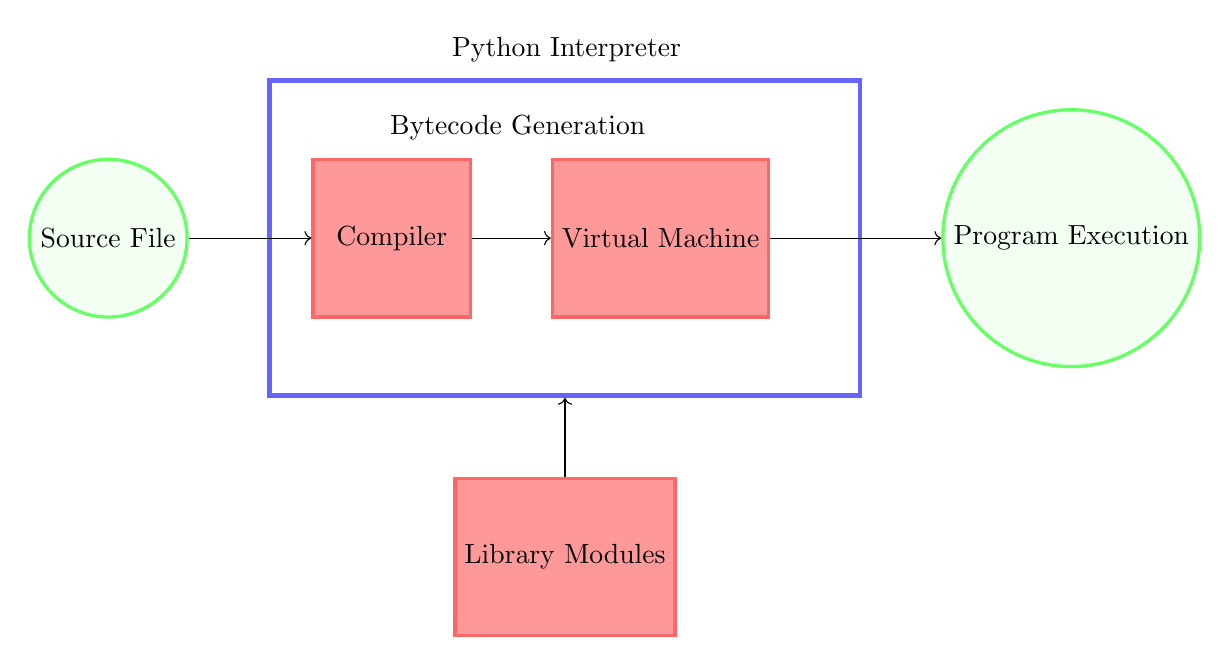
\begin{tikzpicture}
				%% setupP
				[
					roundnode/.style={circle, draw=green!60, fill=green!5, very thick, minimum size=20mm},
					rectanglenode/.style={rectangle, draw=red!60, fill=red!40, very thick, minimum size=20mm},
					transparentbox/.style={rectangle,draw=blue!60, fill=blue!0, ultra thick, minimum width = 75mm, minimum height = 40mm},
				]
					
					%% Nodes
					\node [transparentbox] (box) at (1,0) {};
					\node [rectanglenode] (compilernode) at (-1.2,0){Compiler};
					\node [rectanglenode] (vmnode) [right=of compilernode] {Virtual Machine};
					\node [roundnode] (sourcefile) [left=of box] {Source File};
					\node [roundnode] (programnode) [right=of box] {Program Execution};
					\node [rectanglenode] (librarynode) [below=of box] {Library Modules};
					\node [] (text) at (1.02,2.4) {Python Interpreter};
					\node [] (textBytecode) at (0.4,1.4){Bytecode Generation};
					%% Lines
					\draw[->] (librarynode.north) -- (box.south) ;
					\draw[->] (sourcefile.east) -- (compilernode.west);
					\draw[->] (compilernode.east) -- (vmnode.west);
					\draw[->] (vmnode.east) -- (programnode.west);
				\end{tikzpicture}
			
				\caption{Python Code Execution}
				\label{fig:python code execution}
		\end{figure}
		
		\begin{figure}[h]
			\centering    
			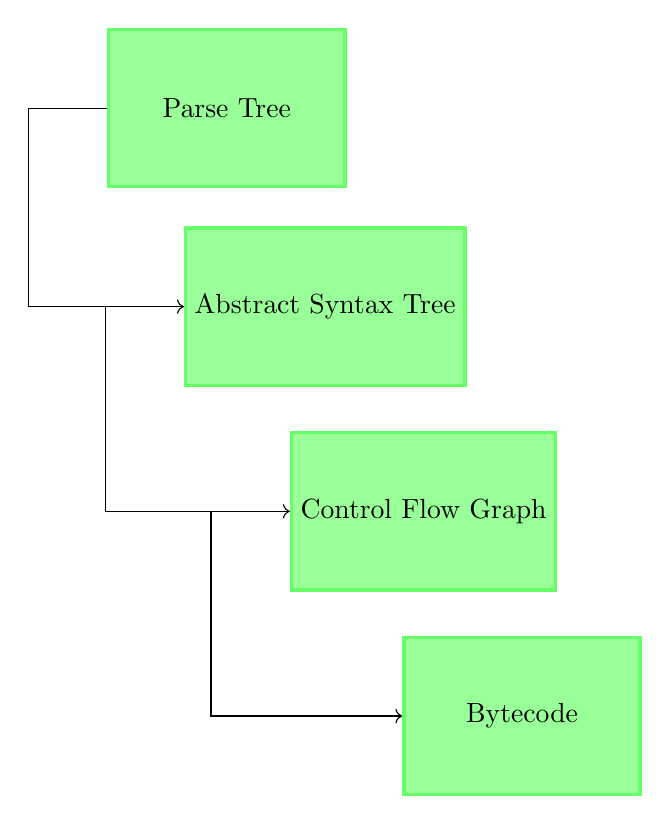
\begin{tikzpicture}
				[
					roundnode/.style={circle, draw=green!60, fill=green!5, very thick, minimum size=20mm},
					rectanglenode/.style={rectangle, draw=green!60, fill=green!40, very thick, minimum width=30mm, minimum height = 20mm},
					transparentbox/.style={rectangle,draw=blue!60, fill=blue!0, ultra thick, minimum width = 75mm, minimum height = 40mm},
				]
				
				\node [rectanglenode] (parsetree) {Parse Tree};
				\node [rectanglenode] (ast) [below=of parsetree] at(1.25,-0.5) {Abstract Syntax Tree};
				\node [rectanglenode] (cfg) [below=of ast] at(2.5,-3.1) {Control Flow Graph};
				\node [rectanglenode] (bytecode) [below=of cfg] at(3.75,-5.7) {Bytecode};

				\draw[->] (parsetree.west) -- ++(-1,0)|- (ast.west) ; 
				\draw[->] (ast.west) -- ++(-1,0)|- (cfg.west) ; 
				\draw[->] (cfg.west) -- ++(-1,0)|- (bytecode.west) ; 

			\end{tikzpicture}
			
			\caption{Compiler Innards}
			\label{fig:compiler_innards}
		\end{figure}

		\begin{figure}[H]
			\centering
			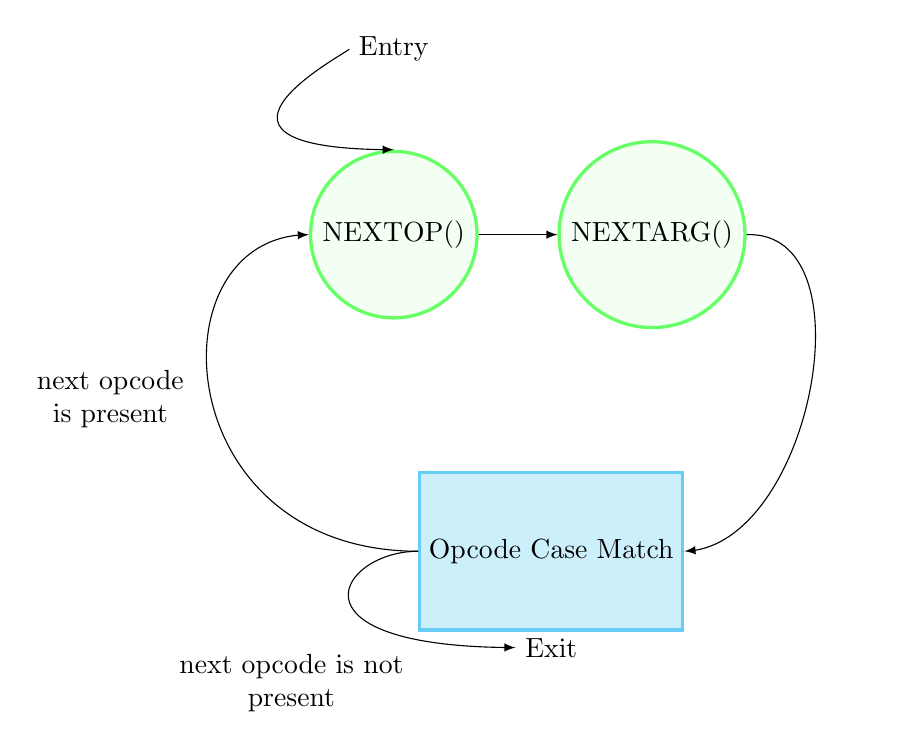
\begin{tikzpicture}
				[
					roundnode/.style={circle, draw=green!60, fill=green!5, very thick, minimum size=20mm},
					rectanglenode/.style={rectangle, draw=cyan!60, fill=cyan!20, very thick, minimum width=30mm, minimum height = 20mm},
					transparentbox/.style={rectangle,draw=blue!60, fill=blue!0, ultra thick, minimum width = 75mm, minimum height = 40mm},
				]

				\node [roundnode] (opcode) {NEXTOP()};
				\node [roundnode] (checkargs) [right=of opcode] {NEXTARG()};
				\node [rectanglenode] (switch) [below=of opcode] at(2,-2) {Opcode Case Match};
				\node [] (entrytext) [above=of opcode] {Entry};
				\node [] (exittext) [below=of switch] at(2,-4) {Exit};
				\node [align=center] (label1) [below=of switch] at(-1.3,-4.2) {next opcode is not\\present};
				\node [align=center] (label2) [below=of switch] at(-3.6,-.6) {next opcode\\is present};
				
				\draw[-latex] (entrytext) .. controls +(left:.5cm) and +(left:3cm) .. (opcode.north);
				\draw[-latex] (switch.west) .. controls +(left:1cm) and +(left:3cm) .. (exittext.west);
				\draw[-latex] (switch.west) .. controls +(left:3.2cm) and +(left:2cm) .. (opcode.west);
				\draw[-latex] (checkargs.east) to[in=1, out=2] (switch.east);
				
				\draw[-latex] (opcode.east) -- (checkargs.west);
				
			\end{tikzpicture}

			\caption{VM Innards}
			\label{fig:vm_innards}
		\end{figure}

		This simple algorithm is known as the CPython Evaluation Loop. The evaluation loop is formulated as shown in Listing \ref{lst:ceval_loop}\footnote{Actual code differs from what is presented. The source code has been edited as to be more readable and concise.}.

		\begin{lstlisting}[float=h,language=Python,caption= Evaluation Loop,label=lst:ceval_loop]
			for(**indefinite condition**){
				oparg=null;
				opcode = NEXTOP();
				if(ARGUMENT_PRESENT(opcode)){
					oparg = NEXTARG();
				}
				switch(opcode){
					case **opcode_name**: 
						manipulate stack & set variables accordingly
					...
					...
					...
					default: 
						raise error
				}
			}	
		\end{lstlisting}

		Evaluation is computed frame by frame (See {\bfseries\nameref{subsec:frames}}), with what is essentially a (very long) switch statement; reading every opcode and delegating accordingly.
			
		\subsection{Stacks}
		\label{subsec:stacks}
		\par A stack data structure is a dynamic structure that operates with a LIFO policy \cite[]{intro2009algorithms}. Since CPython does not directly interact with
		the hardware for compilation, it makes both the call stack and stack frames rely on the PVM. In CPython, there is one main stack that the \acs{PVM} requires for proper functionality; the call stack. 
		The other two stacks (\nameref{subsubsec:value_stack} and \nameref{subsubsec:call_stack}) are essential for the proper computation of any variables that there are in the
		frame (See {{\bfseries\nameref{subsec:frames}}). Most instructions manipulate the value stack and the call stack \cite[]{general2018stacks}. The nature of CPython stacks is visualised in Figure \ref{fig:stacks_overview}
			\subsubsection*{Call Stack}
			\label{subsubsec:call_stack}

			\par The call stack contains call-frames (See {\bfseries\nameref{subsec:frames}}). This is the main structure of the running program.
			A function call results in a pushed frame onto the call stack, whilst 
			a return call results in a pop of the function frame off of the stack \cite[]{call2010stack}. A visual representation of a call stack is shown in Figure \ref{fig:call_stack_example}. 
			In this figure, a sample script can be seen run, step by step, showing the frames being pushed onto the call stack and popped from the call stack.
			The first frame pushed onto the frame stack is inevitably called the \lstinline|__main__| call frame.

			\begin{figure}
				\centering

				\begin{lstlisting}[language=Python,caption=Python script, label=lst:callstackexample]
					def foo():
						print("Hello")
					
					def intermediary():
						foo()
						
					def start():
						intermediary()
					
					start()
				\end{lstlisting}

				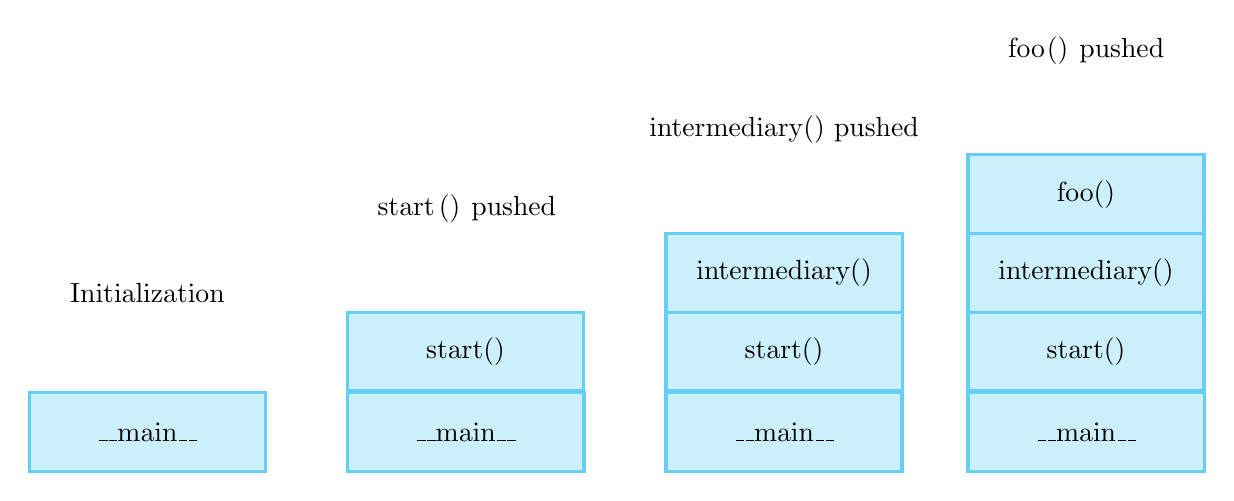
\begin{tikzpicture}
				[
					roundnode/.style={circle, draw=green!60, fill=green!5, very thick, minimum size=20mm},
					rectanglenode/.style={rectangle, draw=cyan!60, fill=cyan!20, very thick, minimum width=30mm, minimum height = 10mm},
					transparentbox/.style={rectangle,draw=blue!60, fill=blue!0, ultra thick, minimum width = 75mm, minimum height = 40mm},
				]
				
				\node[rectanglenode] (main) at (0,0) {\_\_main\_\_};
				\node [] (text_init) [above=of main] {Initialization};
				
				\node[rectanglenode] (main_1) [right=of main] {\_\_main\_\_};
				\node[rectanglenode] (start) [above=of main_1] at (4.04,-0.5) {start()};
				\node [] (text_start) [above=of start] {\lstinline|start()| pushed};

				\node[rectanglenode] (main_2) [right=of main_1] {\_\_main\_\_};
				\node[rectanglenode] (start_2) [above=of main_2] at (8.085,-0.5) {start()};
				\node[rectanglenode] (intermediary) [above=of start_2] at(8.085,0.5) {intermediary()};
				\node [] (text_int) [above=of intermediary] {\lstinline|intermediary()| pushed};
			
				\node[rectanglenode] (main_3) [right=of main_2] at (9.40,0){\_\_main\_\_};
				\node[rectanglenode] (start_3) [above=of main_3] at (11.92,-0.5) {start()};
				\node[rectanglenode] (intermediary_3) [above=of start_3] at(11.92,0.5) {intermediary()};
				\node[rectanglenode] (foo) [above=of intermediary_3] at(11.92,1.5) {foo()};
				\node [] (text_foo) [above=of foo] {\lstinline|foo()| pushed};

				\end{tikzpicture}
				
				\vspace{20mm}

				\begin{tikzpicture}
					[
						roundnode/.style={circle, draw=green!60, fill=green!5, very thick, minimum size=20mm},
						rectanglenode/.style={rectangle, draw=cyan!60, fill=cyan!20, very thick, minimum width=30mm, minimum height = 10mm},
						transparentbox/.style={rectangle,draw=blue!60, fill=blue!0, ultra thick, minimum width = 75mm, minimum height = 40mm},
					]
					
					\node[rectanglenode] (main) at (8.21,0) {\_\_main\_\_};
					\node [] (text_init) [above=of main] {\lstinline|start()| popped};
					
					\node[rectanglenode] (main_1) [right=of main_2] at(1.86,0) {\_\_main\_\_};
					\node[rectanglenode] (start) [above=of main_1] at (4.38,-0.5) {start()};
					\node [] (text_start) [above=of start] {\lstinline|intermediary()| popped};
		
					\node[rectanglenode] (main_2) [right=of main_3] at (-2.3,0){\_\_main\_\_};
					\node[rectanglenode] (start_2) [above=of main_2] at (0.215,-0.5) {start()};
					\node[rectanglenode] (intermediary) [above=of start_2] at(0.215,0.5) {intermediary()};
					\node [] (text_int) [above=of intermediary] {\lstinline|foo()| popped};
				
					\node[rectanglenode] (main_3) at (-3.6,0){\_\_main\_\_};
					\node[rectanglenode] (start_3) [above=of main_3] at (-3.6,-0.5) {start()};
					\node[rectanglenode] (intermediary_3) [above=of start_3] at(-3.6,0.5) {intermediary()};
					\node[rectanglenode] (foo) [above=of intermediary_3] at(-3.6,1.5) {foo()};
					\node [] (text_foo) [above=of foo] at (-3.6,2.5){\lstinline|foo()| computed};
		
				\end{tikzpicture}

				\caption{Simulation of Call Stack running Listing \ref{lst:callstackexample}}
				\label{fig:call_stack_example}

			\end{figure}

			\subsubsection*{Value Stack}
			\label{subsubsec:value_stack}
			\par This stack is also known as the evaluation stack. It is where the manipulation of the object happens when evaluating object-manipulating opcodes.
			A value stack is found in a call-frame, implying bijectivity. Any manipulations performed on this stack (unless they are namespace related) are independent of other stacks and
			do not have the permissions to push values on other value stacks.
			
			\subsubsection*{Block Stack}
			\label{subsubsec:block_stack}

			\par The block stack keeps track of different types of control structures, such as; loops, try/except blocks, and with blocks. These structures push entries onto the block stack, which are popped whenever exiting
			the said structure. The block stack allows the interpreter to keep track of active blocks at any moment

			\begin{figure}
				\centering

				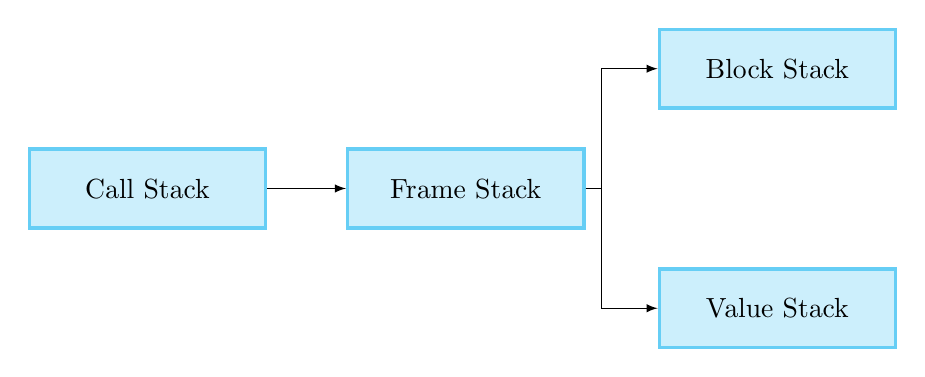
\begin{tikzpicture}
					[
						roundnode/.style={circle, draw=green!60, fill=green!5, very thick, minimum size=20mm},
						rectanglenode/.style={rectangle, draw=cyan!60, fill=cyan!20, very thick, minimum width=30mm, minimum height = 10mm},
						transparentbox/.style={rectangle,draw=blue!60, fill=blue!0, ultra thick, minimum width = 75mm, minimum height = 40mm},
					]

					\node[rectanglenode] (callstack) at (0,0) {Call Stack};

					\node[rectanglenode] (framestack) [right=of callstack] {Frame Stack};
					\node[rectanglenode] (blockstack) [above=of framestack] at (8,0) {Block Stack};
					\node[rectanglenode] (valuestack) [below=of framestack] at (8,0){Value Stack};
					

					\draw[-latex] (callstack) -- (framestack);
					\draw[-latex] (framestack.east) -- ++(0.2,0)|-  (blockstack.west);
					\draw[-latex] (framestack.east) -- ++(0.2,0)|-  (valuestack.west);

				\end{tikzpicture}

				\caption{Overview of CPython stacks}
				\label{fig:stacks_overview}
			\end{figure}

		\pagebreak

		\subsection{Frames}
		\label{subsec:frames}
		\par A frame (call-frame) is an object which represents a current function call (subprogram call); more formally referred to as a code object. It is an internal type containing administrative information useful for debugging and is used
		by the interpreter \cite[pp.18--19]{van1994python}. Frame objects are tightly coupled with the three main stacks (See {\bfseries\nameref{subsec:stacks}}) by which every frame is linked to another. Every frame object has two frame-specific stacks;
		value stack (See {\bfseries\nameref{subsubsec:value_stack}}) and the block stack (See {\bfseries\nameref{subsubsec:block_stack}}). Frames are born from function calls, and die when that function is returned.
		
			\subsubsection*{Frame Attributes}
			\par Along with the properties mentioned above, a frame object would have the following attributes:
			\begin{description}
				\item [f\_back] points to the previous stack frame object (return address).
				\item [f\_code] points to the current code object (See {\bfseries\nameref{subsec:code_obj}}) being executed, in the current frame.
				\item [f\_builtin] points to the builtin symbol table.
				\item [f\_globals] points to the dictionary used to look up global variables.
				\item [f\_locals] points to the symbol table used to look up local variables.
				%\item [f\_valuestack] this is a pointer, which points to the address after the last local variable. TODO:WRONG
				\item [f\_valuestack] this holds the pointer, pointing to the value of the top of the value stack.
				\item [f\_lineno] this gives the line number of the frame.
				\item [f\_lasti] this gives the bytecode instruction offset of the last instruction called.
				\item [f\_blockstack] contains the block state, and block relations.
				\item [f\_localsplus] is a dynamic structure that holds any values in the value stack, for evaluation purposes.
			\end{description}

			These attributes are retrieved from the declaration found in \textit{./Include/frameobject.h}.

			\subsubsection*{Frame Stack}
			\par The stack frame is a collection of all the current frames in a call-stack-like data structure (See {\bfseries\nameref{subsubsec:call_stack}}).
			A frame is pushed onto the stack frame for every function call (every function has a unique frame) as shown in Figure \ref{fig:stack_frames}.
			\par The stack frame contains a frame pointer which is another register that is set to the current stack frame. Frame pointers resolve the issue created 
			when operations (pushes or pops) are computed on the stack hence changing the stack pointer, invalidating any hard-coded offset addresses that are computed statically, before run-time \cite[]{stack2011csuwm}.
			With frame pointers, references to the local variables are offsets from the frame pointer, not the stack pointer.
			\begin{figure}[H]
				
				\centering
				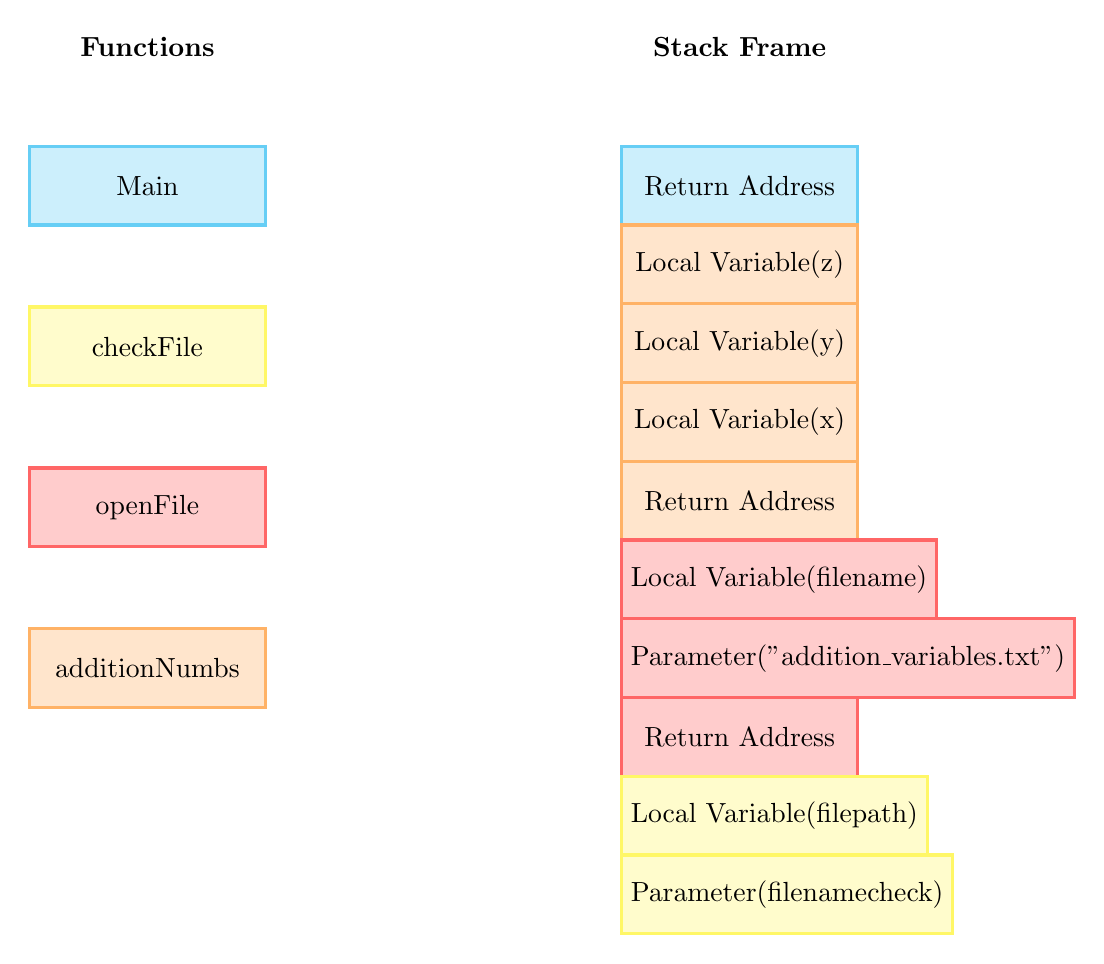
\begin{tikzpicture}
					[
						roundnode/.style={circle, draw=green!60, fill=green!5, very thick, minimum size=20mm},
						rectanglenode_main/.style={rectangle, draw=cyan!60, fill=cyan!20, very thick, minimum width=30mm, minimum height = 10mm},
						rectanglenode_checkFile/.style={rectangle, draw=yellow!60, fill=yellow!20, very thick, minimum width=30mm, minimum height = 10mm},
						rectanglenode_openFile/.style={rectangle, draw=red!60, fill=red!20, very thick, minimum width=30mm, minimum height = 10mm},
						rectanglenode_addition/.style={rectangle, draw=orange!60, fill=orange!20, very thick, minimum width=30mm, minimum height = 10mm},
						transparentbox/.style={rectangle,draw=blue!60, fill=blue!0, ultra thick, minimum width = 75mm, minimum height = 40mm},
					]
					
					
					\node[rectanglenode_main] (mainfunc) at (0,0) {Main};
					\node[rectanglenode_checkFile] (func1) [below=of mainfunc] {checkFile};
					\node[rectanglenode_openFile] (func2) [below=of func1] {openFile};
					\node[rectanglenode_addition] (func3) [below=of func2] {additionNumbs};
					
					\node[rectanglenode_main] (mainfunc_frame1) [right= of mainfunc] at (5,0) {Return Address};
					\node[rectanglenode_addition] (addition_frame1) [right= of mainfunc] at (5,-1) {Local Variable(z)};
					\node[rectanglenode_addition] (addition_frame1) [right= of mainfunc] at (5,-2) {Local Variable(y)};
					\node[rectanglenode_addition] (addition_frame1) [right= of mainfunc] at (5,-3) {Local Variable(x)};
					\node[rectanglenode_addition] (addition_frame1) [right= of mainfunc] at (5,-4) {Return Address};
					\node[rectanglenode_openFile] (openFile_frame1) [right= of func1] at(5,-5){Local Variable(filename)};
					\node[rectanglenode_openFile] (openFile_frame2) [right= of func1] at(5,-6){Parameter("addition\_variables.txt")};
					\node[rectanglenode_openFile] (openFile_frame3) [right= of func1] at(5,-7){Return Address};
					\node[rectanglenode_checkFile] (checkFile_frame1) [right= of func1] at(5,-8){Local Variable(filepath)};
					\node[rectanglenode_checkFile] (checkFile_frame2) [right= of func1] at(5,-9){Parameter(filenamecheck)};
					
					\node[] (textfunctions) [above=of mainfunc] {\bfseries{Functions}};
					\node[] (textstack) [above=of mainfunc_frame1] {\bfseries{Stack Frame}};

				\end{tikzpicture}
				\caption{Stack frames example}
				\label{fig:stack_frames}
			
			\end{figure}

		\subsection{Code Objects}
		\label{subsec:code_obj}
		
		\par A code object is a low-level detail of the CPython implementation. When parsing Python code, compilation creates a code object for processing on the \acs{PVM}. A code object contains a list of instructions directly interacting with the CPython \acs{VM}; hence coined a low-level detail. Code objects are of the type \lstinline|PyCodeObject|, with each section of the code object representing 
		a chunk of executable code that has not been bound to a function \cite[]{pythonofficial2022docspycode}. The structure of the type of these code 
		objects change throughout different CPython versions, thus there is no set composition \cite[]{pythonofficial2022docspycode}. For reference, the source code in Listing \ref{lst:dis_example} produces
		the code object displayed in Listing \ref{lst:codeobjscript}, following the standard convention shown in Listing \ref{lst:codeobjconv}.
		
		\begin{lstlisting}[float=h,language=bash, caption= Code object of Listing \ref{lst:dis_example},numbers=none]
			<code object addition_numbers at 0x1047f10b0, file "filepath", line 3>
		\end{lstlisting}\label{lst:codeobjscript}
		
		\small
		\begin{lstlisting}[float=h,language=bash, caption= Code object standard convention,numbers=none]
			code object <functionName> at <address>, file <path>, line<firstLineNo.>
		\end{lstlisting}\label{lst:codeobjconv}
		
		\normalsize

			\subsubsection*{Disassembler}
			\par Code objects are expanded by using the \lstinline|dis| module in Python. This module contains several analyses functions which; all of which directly convert the input code object into the desired output \cite[]{pythonofficial2022docsdismodule}.
			The function that is of a particular interest in this paper is the \lstinline|dis.dis| function which disassembles a code object into its respective bytecodes, alongside other relevant information, as seen in Figure \ref*{lst:dis_example}.
			When applying the analysis function \lstinline|dis.dis|, the disassembled code object takes the following format for every instruction:
			
			\small
			\begin{lstlisting}[language=bash, caption= Dissasembled instruction convention,numbers=none]
				<lineNumber><label><instructionOffset><opname><opargs><var>
			\end{lstlisting}
			\normalsize

			It is interesting to note that the value for \lstinline|opargs| is computed in little-endian order. Typically, as is shown in ... ,the arguments associated with the instructions are used for 
			specific stack manipulations. 
			%%TODO: Maybe add some more detail
			%%TODO: Add the correct reference section above.

				
				\begin{lstlisting}[language=Python,caption=Python source code,label=lst:addnossource]
				        import dis
				        
				        def addition_numbers(x,y):
				            z=x+y
				            return z
				       
				        dis.dis(addition_numbers)
				\end{lstlisting}

				\begin{lstlisting}[numbers=none, caption=Disassembly of Listing \ref{lst:addnossource}]
				4    	0 LOAD_FAST        0(x)
							2 LOAD_FAST        1(y)
							4 BINARY_ADD
							6 STORE_FAST       2(z)
				
				5		  LOAD_FAST        2(z)
							10 RETURN_VALUE
				\end{lstlisting}\label{lst:dis_example}
%			\end{figure}

			\subsubsection*{Bytecode}
			\label{subsubsec:bytecode}
			
			\par Bytecode is a form of portable code (p-code) executed on a virtual machine. 
			The introduction of the concept of bytecode came about when a generalized way 
			 of interpreting complex programming languages was required to simplify information structures, characterizing them in their essentials \cite[]{landin1964mechanical}.
			 This ideology gave birth to portable code; a generalized form of code, that can cross-compile, assuming that
			 the Virtual Machine which interpreted the p-code was compatible with the native machine architecture. 
			 \par In CPython V3.10, there are over 100 low-level bytecode instructions \cite[]{pythonofficial2022docsdismodule}. The classification of bytecode operations is defined below:
			\begin{itemize}
				\item[-]Unary instructions.
				\item[-] Binary instructions.
				\item[-] Inplace instructions.
				\item[-] Coroutine instructions.
				\item[-] Argument instructions.
				\item[-] Miscellaneous instructions.
			\end{itemize}
			
		\subsection{Execution of Code Objects}
		The evaluation stage firstly makes use of the public API \lstinline|PyEval_EvalCode()| \cite[lines 716--724]{ceval2022github}, which is used for evaluating a code object created 
		at the end of the compilation stages (Figure \ref{fig:compiler_innards}). This API constructs an execution frame from the top of the stack by calling \lstinline|_PyEval_EvalCodeWithName()|.
		The first execution frame constructed must conform to these requirements:
		\begin{enumerate}
			\item The resolution of keyword\footnote{A keyword argument is a value that, when passed into a function, is identifiable by a specific parameter name, such as variable assignment.} 
			and positional arguments\footnote{A positional argument is a value that is passed into a function based on the order in which the parameters were listed during the function definition.}.
			\item The resolution of *args\footref{footnote:kwargs_args} and **kwargs\footnote{\label{footnote:kwargs_args}*args and **kwargs allow multiple arguments to be passed into a function via the unpacking (*) operator.} 
			in function definitions.
			\item The addition of arguments as local variables to the scope (A scope is the membership of a variable to a region).
			\item The creation of Co-routines and Generators \cite[pp.2--3]{tismer2000continuations}.
		\end{enumerate} 
		Code execution in CPython is the evaluation and interpretation of code object. Below, we delve into a more detailed description of frame objects; their creation, and execution \cite[]{real2022python}.
		
			\subsubsection*{Thread State Construction}
			\par Prior to execution, the frame would need to be referenced from a thread. The interpreter allows for many threads to run at any given moment. The thread structure that is created is called 
			\lstinline|PyThreadState|.
			
			\subsubsection*{Frame Construction}
			\par Upon constructing the frame, the following arguments are required:
			\begin{description}
				\item [\_co] A \lstinline|PyCodeObject| (code object).
				\item [globals] A dictionary relating global variable names with their values.
				\item [locals] A dictionary relating local variable names with their values.
			\end{description}
			It is important to note that there are other arguments that might be used but do not form part of the basic API, thus will not be included.

			\subsubsection*{Keyword \& Positional Argument Handling}
			\par If the function definition contains a multi-argument keyword argument \footref{footnote:kwargs_args}, a new keyword argument dictionary (\lstinline|kwdict| dictionary) is created in the form of a \lstinline|PyDictObject|.
			Similarly, if any positional arguments\footref{footnote:kwargs_args} are found they are set as local variables.

			\par The dictionary that was created is now filled with the remaining keyword arguments which do not resolve themselves to positional arguments. This resolution comes after
			all the other arguments have been unpacked. In addition, missing positional arguments \footnote{Positional arguments that are provided to a function call, but are not in the list of positional arguments.} are 
			added to the \lstinline|*args|\footref{footnote:kwargs_args} tuple. The same process is followed for the keyword arguments; values are added to the \lstinline|**kwargs| dictionary and not a tuple.

			\subsubsection*{Final Stage}
			\par Any closure names are added to the code object's list of free variable names, and finally, generators and coroutines are handled in a new frame. In this case, the frame is not pre-evaluated but it is 
			evaluated only when the generator/coroutine method is called to execute its target.


		\subsection{Execution of Frame Objects}
		\par The local and global variables are added to the frame preceding frame evaluation; handled by \lstinline|_PyEval_EvalFrameDefault()|. 
		\par\lstinline|_PyEval_EvalFrameDefault()| is the central function which is found in the main execution loop. Anything that CPython executes goes through
		this function and forms a vital part of interpretation.
    
	%\chapter{User Manual}
\Blindtext
 




\end{document}

%%% The End %%%
